% La parte central del trabajo refiere a lo que es producción propia o aporte del
% proyecto de grado, incluyendo las decisiones tomadas. Por ejemplo, puede incluir
% los requerimientos, el análisis y el diseño de la solución. Si el proyecto tiene una
% implementación, debe describirse en términos de decisiones tomadas en ese sentido.
% Los detalles de programación se dejan para los anexos.

% Se pueden incluir figuras en el documento, las mismas deben estar referenciadas en el texto. Por ejemplo, la Figura~\ref{fig:logos} muestra los logos de Facultad de Ingeniería y de la Universidad de la República.

% \begin{figure}[h!]
%     \centering
%     
\includegraphics[width=\textwidth]{figs/logo-udelar-fing.png}
%     \caption{Logos de FIng y UdelaR}
%     \label{fig:logos}
% \end{figure}

\graphicspath{{chapters/3_diseño/figures/}}

% parte central
\chapter{Voxel cone tracing}\label{chap:design}

En este capítulo se detalla el diseño de \textit{voxel cone tracing} \cite{voxel-cone-tracing}, un algoritmo de iluminación global en tiempo real, que utiliza conceptos presentes en el trazado de rayos (\ref{sec:ray-tracing}), trazado de conos (\ref{sec:historical-cone-tracing}) y \textit{photon mapping} (\ref{sec:photon-mapping}), 
pero reduciendo los costos asociados a estos algoritmos clásicos usando una representación de la escena con vóxeles (\ref{sec:voxels}), almacenada en un \textit{octree} disperso (\ref{sec:octree}), para aproximar los conos.

Otra forma de reducir costos y aumentar la velocidad del algoritmo es utilizando el ducto de rasterización \ref{sec:graphics-pipeline} y renderizado diferido \ref{sec:deferred-rendering}.
Los cálculos de luz se realizan en el \textit{fragment shader} del ducto de raster, sobre los \textit{geometry buffers} para reducir la cantidad de fragmentos o hilos de la GPU sobre los que se corren calculos pesados, sin perder calidad de imagen.
Lo anteriormente explicado difiere del trazado de rayos clásico, que renderiza toda la escena puramente mediante intersecciones entre rayos y geometría.

La principal aproximación que realiza este algoritmo es trabajar sobre una representación voxelizada pre-filtrada de la escena.
Dadas las coordenadas de un punto de la escena, se recorre el árbol para hallar el vóxel que representa la región del espacio que incluye ese punto.
Este vóxel contiene toda la información necesaria sobre oclusión, color e irradiancia debido a que la estructura es previamente filtrada.
En el filtrado, la información en las hojas del árbol es promediada hacia niveles mayores hasta que cada nivel del árbol contiene información que aproxima las capas inferiores.
La información de un vóxel en cada nivel resume la información de los vóxeles de los nodos hijos que comparten el mismo espacio en la escena.
Se vió en la sección sobre trazado de conos (\ref{sec:ray-tracing}), que en su planteo original, se hallaban las intersecciones del cono con los objetos de la escena de manera analítica, lo que es costoso.
Aquí, en lugar de hallar la intersección analiticamente, se aproxima el cono utilizando la estructura jerárquica de vóxeles, permitiendo acumular la información a lo largo del cono mas eficientemente, pero con cierta perdida de detalle.

El algoritmo se puede dividir en 4 grandes etapas:

\begin{enumerate}
    \item Voxelización de la escena
    \item Construcción y filtrado del \textit{octree} disperso
    \item Inyección de fotones
    \item Trazado de conos
\end{enumerate}

La voxelización, la inyección de fotones y el trazado de conos usan el ducto de rasterización, mientras que la construcción del árbol y el filtrado usan el ducto de cómputo de propósito general.
En el resto del capítulo se explicará con mayor grado de detalle cada una de estas etapas.

\section{Voxelización}\label{sec:voxelization}

La escena se divide en una grilla de vóxeles.
La cantidad de vóxeles es configurable, siendo usualmente $512$ o $1024$ por dimensión, totalizando $512^3$ o $1024^3$ vóxeles respectivamente.
Un ejemplo de voxelización se muestra en la figura \ref{fig:voxelized-cow}, con $64$, $128$ y $256$ vóxeles por dimensión.

\begin{figure}[ht]
    \begin{subfigure}{.50\textwidth}
        \centering
        \begin{subfigure}{.60\textwidth}
            \centering
            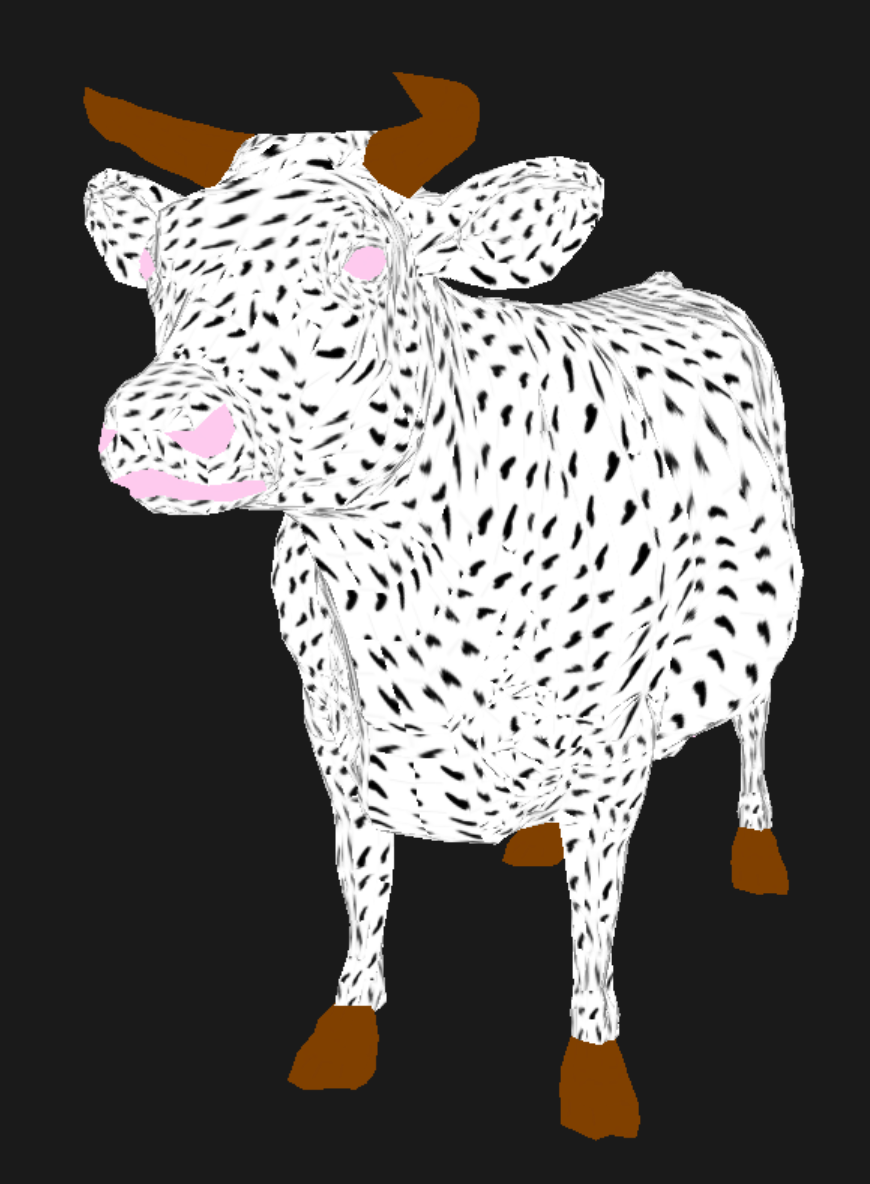
\includegraphics[width=\textwidth]{cow.png}
            \caption{No voxelizado.}
        \end{subfigure}
    \end{subfigure}
    \begin{subfigure}{.50\textwidth}
        \centering
        \begin{subfigure}{.60\textwidth}
            \centering
            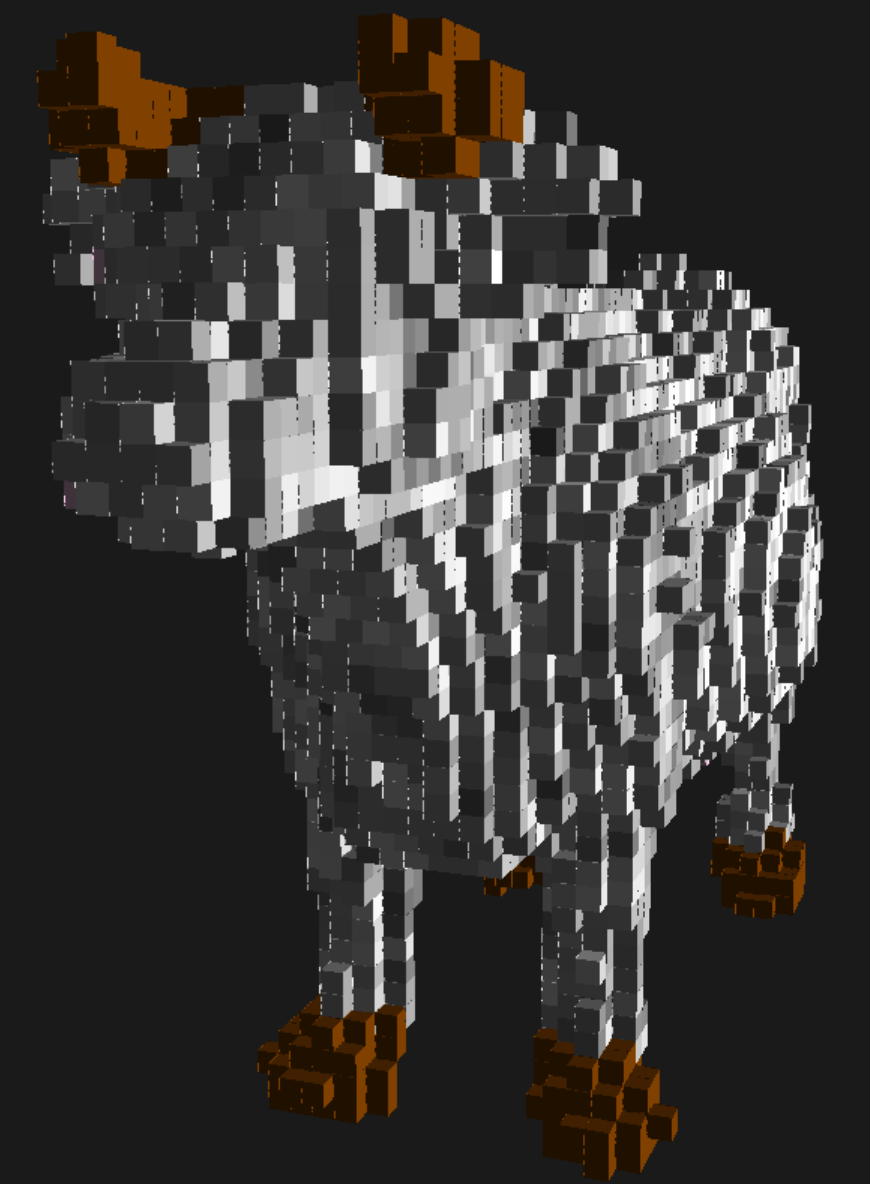
\includegraphics[width=\textwidth]{cow-voxels-64.png}
            \caption{Voxelizado ($64^3$).}
        \end{subfigure}
    \end{subfigure}
    \begin{subfigure}{.50\textwidth}
        \centering
        \begin{subfigure}{.60\textwidth}
            \centering
            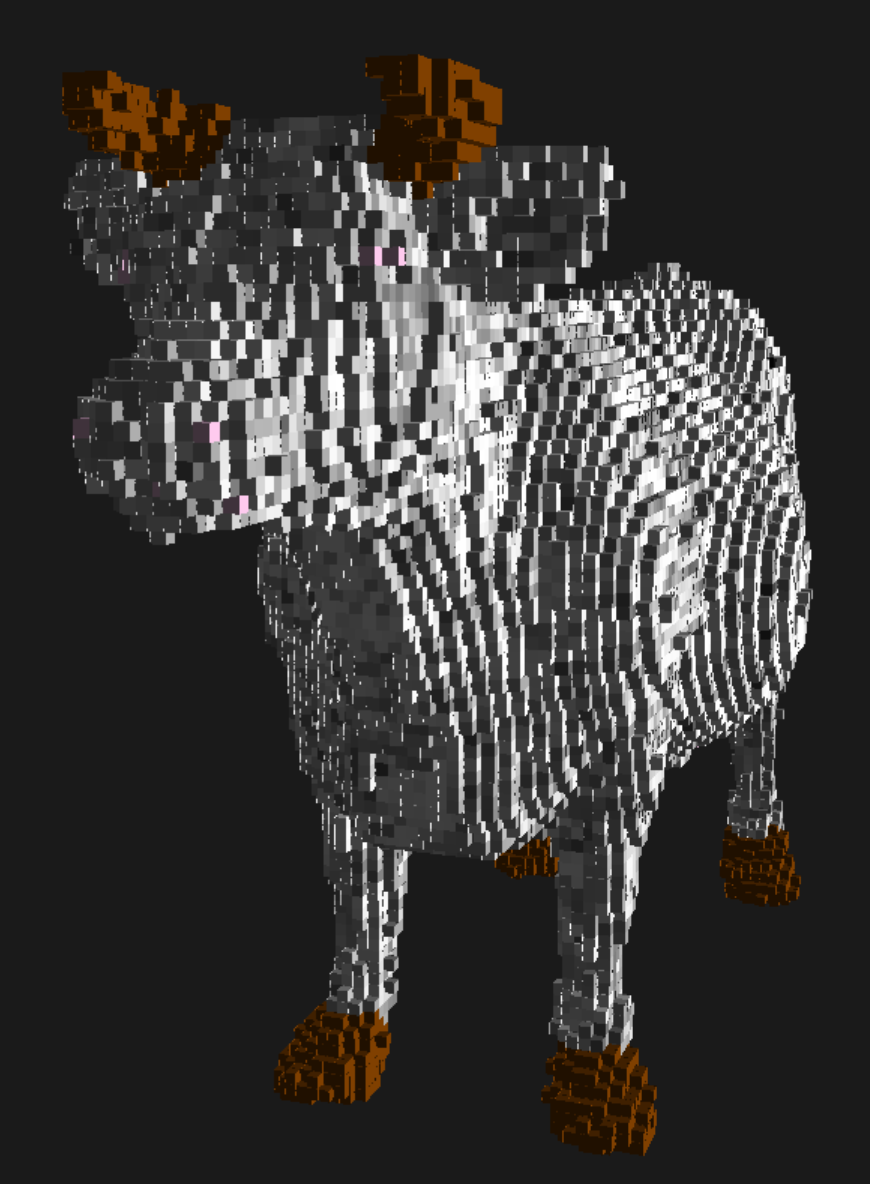
\includegraphics[width=\textwidth]{cow-voxels-128.png}
            \caption{Voxelizado ($128^3$).}
        \end{subfigure}
    \end{subfigure}
    \begin{subfigure}{.50\textwidth}
        \centering
        \begin{subfigure}{.60\textwidth}
            \centering
            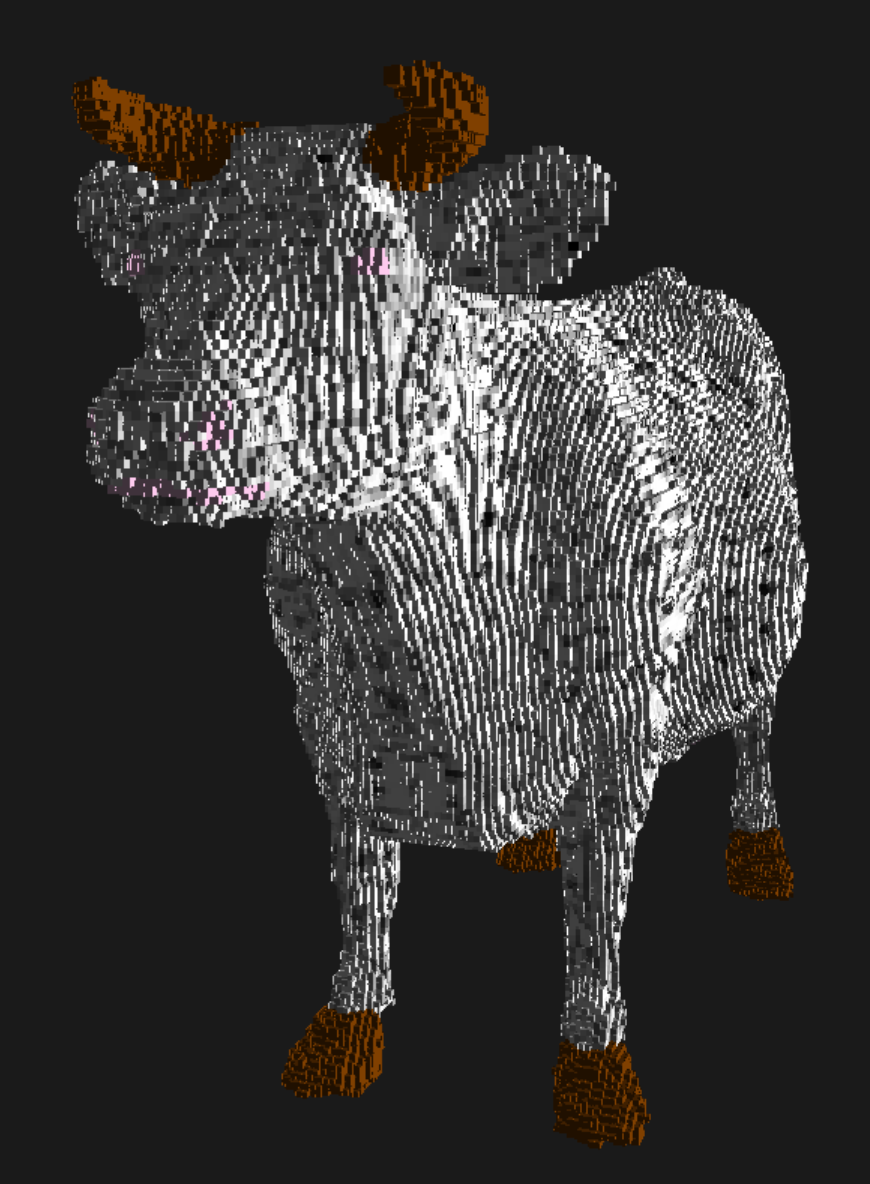
\includegraphics[width=\textwidth]{cow-voxels-256.png}
            \caption{Voxelizado ($256^3$).}
        \end{subfigure}
    \end{subfigure}
    \caption{Ejemplo de voxelización con la cantidad de vóxeles por dimensión entre paréntesis.}
    \label{fig:voxelized-cow}
\end{figure}

Para voxelizar la escena, se realiza el procedimiento detallado en ``OpenGL Insights, capítulo 22'' \cite{opengl-insights}, un aporte escrito por Crassin luego de haber publicado el artículo de \textit{voxel cone tracing}, aprovechando mejoras en las herramientas disponibles en el momento.
Ese mismo proceso será explicado a continuación, para más información, consultar la referencia.

Usando el ducto de rasterización de OpenGL, se procesan todos los triángulos de la geometría de la escena utilizando como resolución para el rasterizado la resolución de la grilla de vóxeles.
Esto genera una lista de \textbf{vóxeles}, donde cada vóxel es una posición dentro de la grilla y un color, que es el color de un triangulo que interseca con el espacio representado por el vóxel.
Cada uno de estos vóxeles será usado para construir el árbol y terminará almacenado en la estructura. Dado lo anteriormente descrito, el mismo vóxel, identificado por su posición en la grilla, puede estar presente en al lista multiples veces con colores diferentes si mas de un triangulo interseca con el vóxel. 

La voxelización de un triángulo $B$ a un vóxel $V$ puede hacerse si:

\begin{enumerate}
    \item El plano de $B$ interseca $V$.
    \item La proyección 2D del triángulo $B$ por la dimensión dominante de su normal (la que provee la mayor área proyectada) interseca la proyección 2D de $V$.
\end{enumerate}

Basado en esta observación, se sigue la serie de pasos que se muestra en la figura \ref{fig:voxelization_pipeline}.

\begin{figure}[h!]
    \centering
    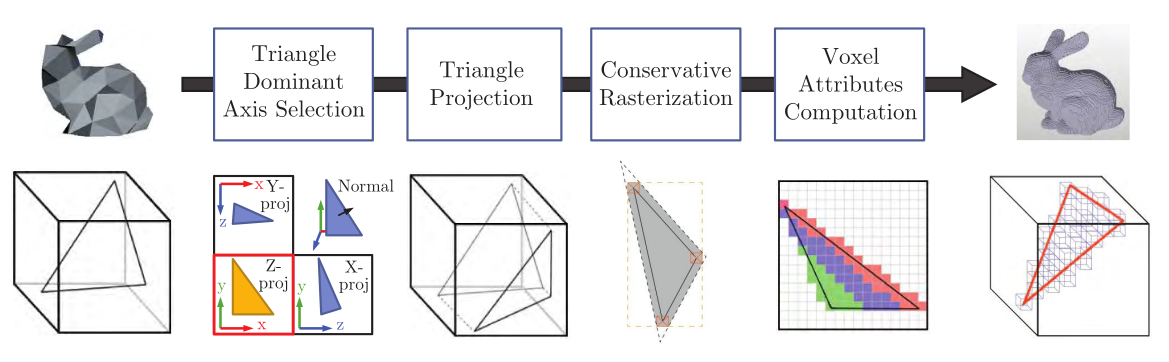
\includegraphics[width=\textwidth]{voxelization_pipeline.png}
    \caption{Ducto de voxelización. Fuente: \cite{opengl-insights}.}
    \label{fig:voxelization_pipeline}
\end{figure}

Primero, cada triángulo de la geometría se proyecta ortográficamente en la dimensión dominante de su normal.
La dimensión dominante se elige dinámicamente por triángulo en el \textit{geometry shader}, donde la información de los tres vértices de cada triángulo está disponible,
maximizando el area del triangulo proyectado.

Cada triángulo proyectado se rasteriza para conseguir fragmentos correspondientes a la resolución 2D de la grilla de vóxeles.
Se fija el tamaño del \textit{viewport} a coincidir con la cantidad de vóxeles, por ejemplo un \textit{viewport} de tamaño $512\times512$ para una grilla de $512^3$ vóxeles.
% Mientras se hace esto, se mantienen las operaciones del framebuffer desactivadas, como el depth testing. % TODO: Habría que explicar por qué, no entendí del capítulo de OpenGL Insights. No se por que se desactiva el depth testing, si igual lo que se genera en el frame buffer no se usa, suena como algo de bajo nivel

Durante la rasterización, cada triángulo genera un conjunto de fragmentos 2D.
Estos fragmentos generarian solo un vóxel en la grilla si esta fuese 2D, sin embargo al ser una grilla 3D, un triangulo cuyo plano no es perpendicular a su dirección dominante puede intersecar con mas de un vóxel en la dirección de proyección(profundidad).

Es necesario calcular la intersección del plano del triangulo con los vóxeles para encontrar los valores de profundidad en la grilla, ya que el triángulo fue proyectado perdiendo sus valores de profundidad.
Debido a la elección de la dimensión dominante de la normal para la proyección del triangulo, cada fragmento puede generar de 1 a 3 vóxeles con mismos valores de $x$ e $y$ pero diferentes valores de $z$, fuese $z$ la dirección dominante. % TODO: Por qué? No se explicarlo sin algun dibujo :sweat-smile: Yo tampoco, asi que voy a agregar dibujitos o dejarlo para que nos pregunten porque creo que es de lo que mas me cuesta explicar
Entonces, por cada fragmento 2D, los vóxeles que intersecan con el triángulo se calculan en el \textit{fragment shader}, basándose en la posición, la profundidad y las derivadas de la profundiad en espacio de pantalla. % Hacemos lo de las derivadas? Si!
Se necesitan la derivadas para calcular la orientación del plano del triángulo, ya que los fragmentos no tiene información global del triangulo que los genero, solo datos del punto responsable de la generación del mismo.

Luego de realizada la voxelización, se obtiene la lista de vóxeles necesaria para crear el árbol, con su posición y color.
Cada uno tiene sus coordenadas en $\mathbb{N}^3$ que lo identifica dentro de la grilla 3D de la escena, así como color.
Su posición en el espacio de la escena se pude calcular a partir de su posición en la grilla.

\subsection{Rasterización conservativa}

El método descrito anteriormente a veces no crea vóxeles para elementos muy finos, como un asta de bandera, ya que en el rasterizado solo se prueba el centro del píxel contra los triángulos para generar fragmentos.
Se necesita una manera de generar fragmentos para cada píxel tocado por un triángulo, no necesariamente en el centro.
Un algoritmo así se detalla en \cite{conservative-rasterization}.

La idea es generar, por cada triángulo, un polígono acotante ligeramente más grande, para asegurarse que cualquier triángulo proyectado que interseca con cualquier punto del píxel también interseque con su centro.
Se logra trasladando las aristas del triángulo hacia afuera, la mitad de la diagonal de un píxel, y extendiendolas para generar un triangulo semejante.
A su vez se generan fragmentos nuevos que resultan de sobreestimar la cobertura de este triángulo, dado que este nuevo triangulo puede intersecar con el centro de píxeles que antes no intersecaban en ningun punto.
Para evitar estos fragmentos también se genera una caja acotante alineada con los ejes, y se descartan fragmentos por fuera de la misma.
Este proceso se muestra en la figura \ref{fig:conservative_rasterization}.

\begin{figure}[h!]
    \centering
    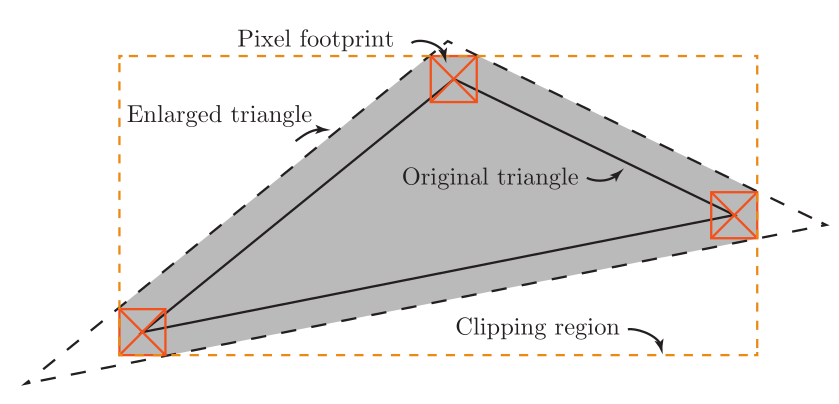
\includegraphics[width=\textwidth]{conservative_rasterization.png}
    \caption{Rasterización conservativa. Fuente: \cite{opengl-insights}.}
    \label{fig:conservative_rasterization}
\end{figure}

\section{\textit{Octree} disperso}

Para almacenar los vóxeles generados, se usa un \textit{octree} disperso, como los vistos en la sección \ref{sec:octree}.
Un octree denso subdivide la escena en 8 cubos y cada cubo se subdivide en 8, y asi sucesivamente. Esta estructura escala rápidamente, generando problemas importante de volumen y velocidad de acceso necesarios a memoria.
Para alivianar este problema se crearon los \textit{octrees} dispersos, donde los nodos no se subdividen si no poseen geometría dentro.

Cada elemento del árbol es un \textbf{nodo}.
Un nodo del árbol representa una sección de la escena.
Cada nivel tiene una cierta cantidad de nodos.
En un árbol denso, cada nodo no hoja tiene exactamente 8 hijos, por lo que cada nivel $n$ tendría $8^n$ nodos.
El nivel $0$ tiene $2^{(0\times 3)} = 1$ nodo, el nivel $1$ tiene $2^{(1\times 3)} = 8$, el $2$ tiene $2^{(2\times 3)} = 64$ y así sucesivamente. % Esto se desprende de lo anterior, pero me parece una simplificacion posiblemente util
El último nivel del árbol es el que llega a la resolución deseada de $512$ o $1024$ vóxeles.
Valores más altos de resolución crean más niveles del \textit{octree} y hacen que la aproximación de vóxeles se asemeje cada vez más a la malla de triángulos original.

En la figura \ref{fig:octree-levels}, se muestra un modelo al que luego de ser voxelizado, se creó un \textit{octree} disperso.
La resolución utilizada fue de $128$ vóxeles por dimensión, por lo que el último nivel del \textit{octree} es el 7.
En la figura se muestran los niveles 5, 6 y 7.

\begin{figure}[ht]
    \begin{subfigure}{.24\textwidth}
        \centering
        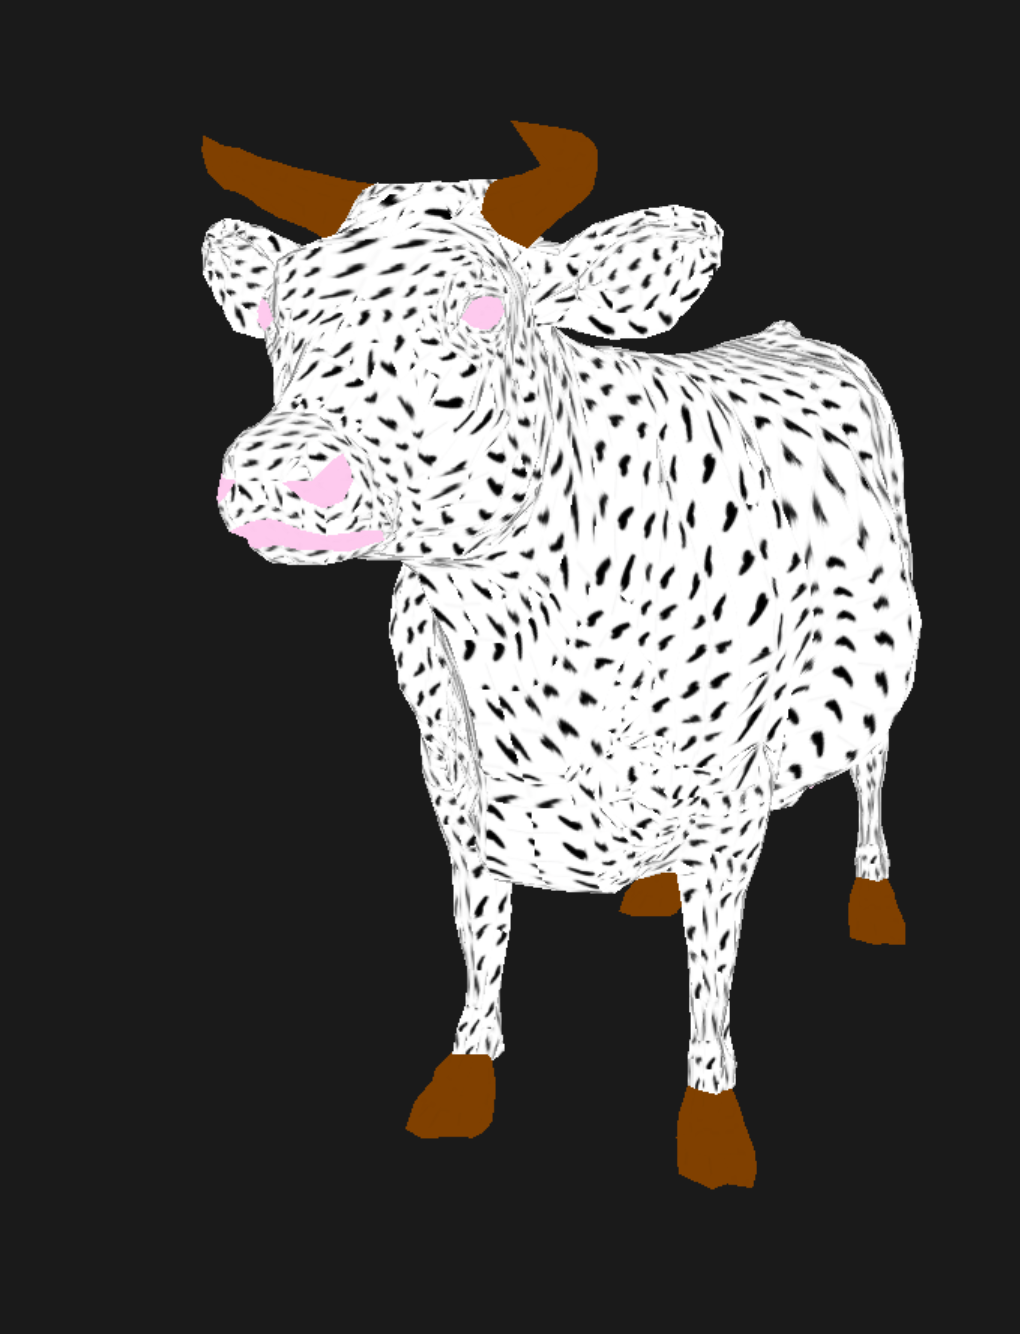
\includegraphics[width=\textwidth]{cow-other-angle.png}
        \caption{Modelo.}
    \end{subfigure}
    \begin{subfigure}{.24\textwidth}
        \centering
        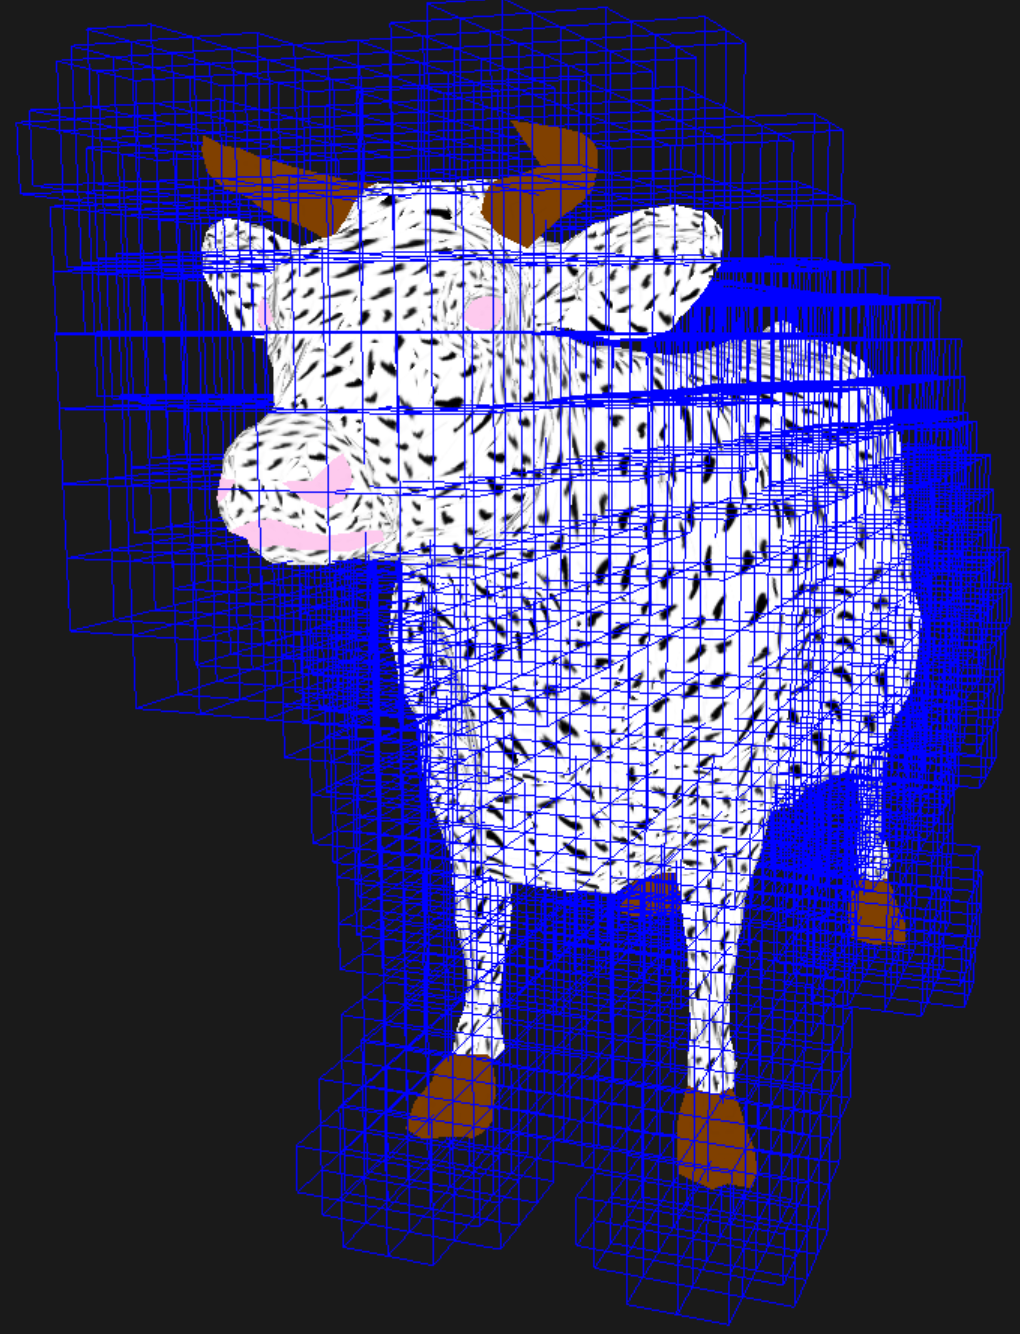
\includegraphics[width=\textwidth]{cow-octree-5.png}
        \caption{Octree nivel 5.}
    \end{subfigure}
    \begin{subfigure}{.24\textwidth}
        \centering
        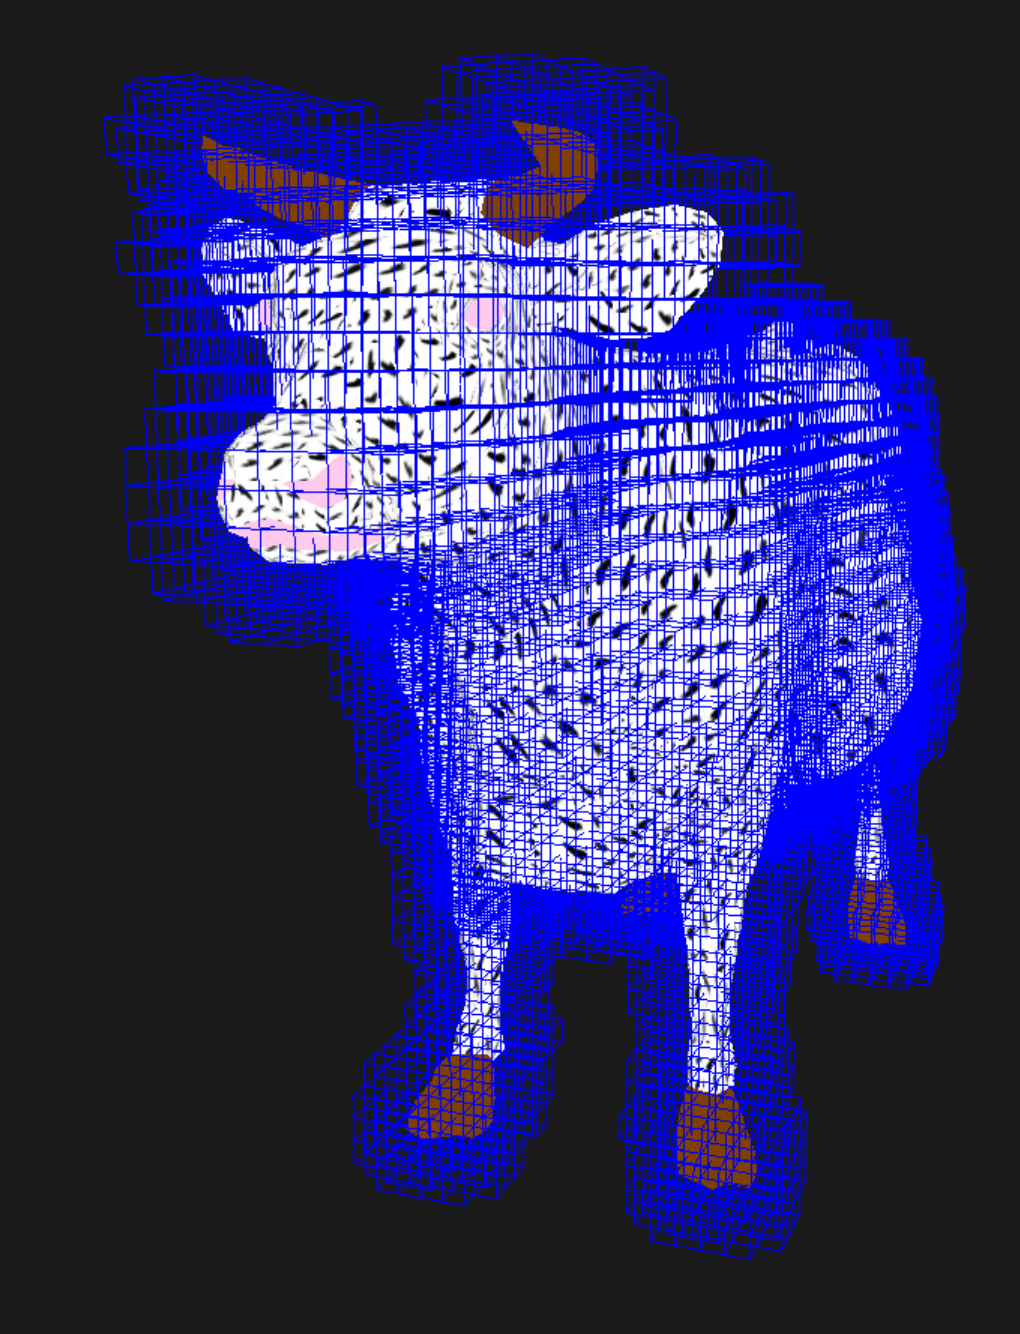
\includegraphics[width=\textwidth]{cow-octree-6.png}
        \caption{Octree nivel 6.}
    \end{subfigure}
    \begin{subfigure}{.24\textwidth}
        \centering
        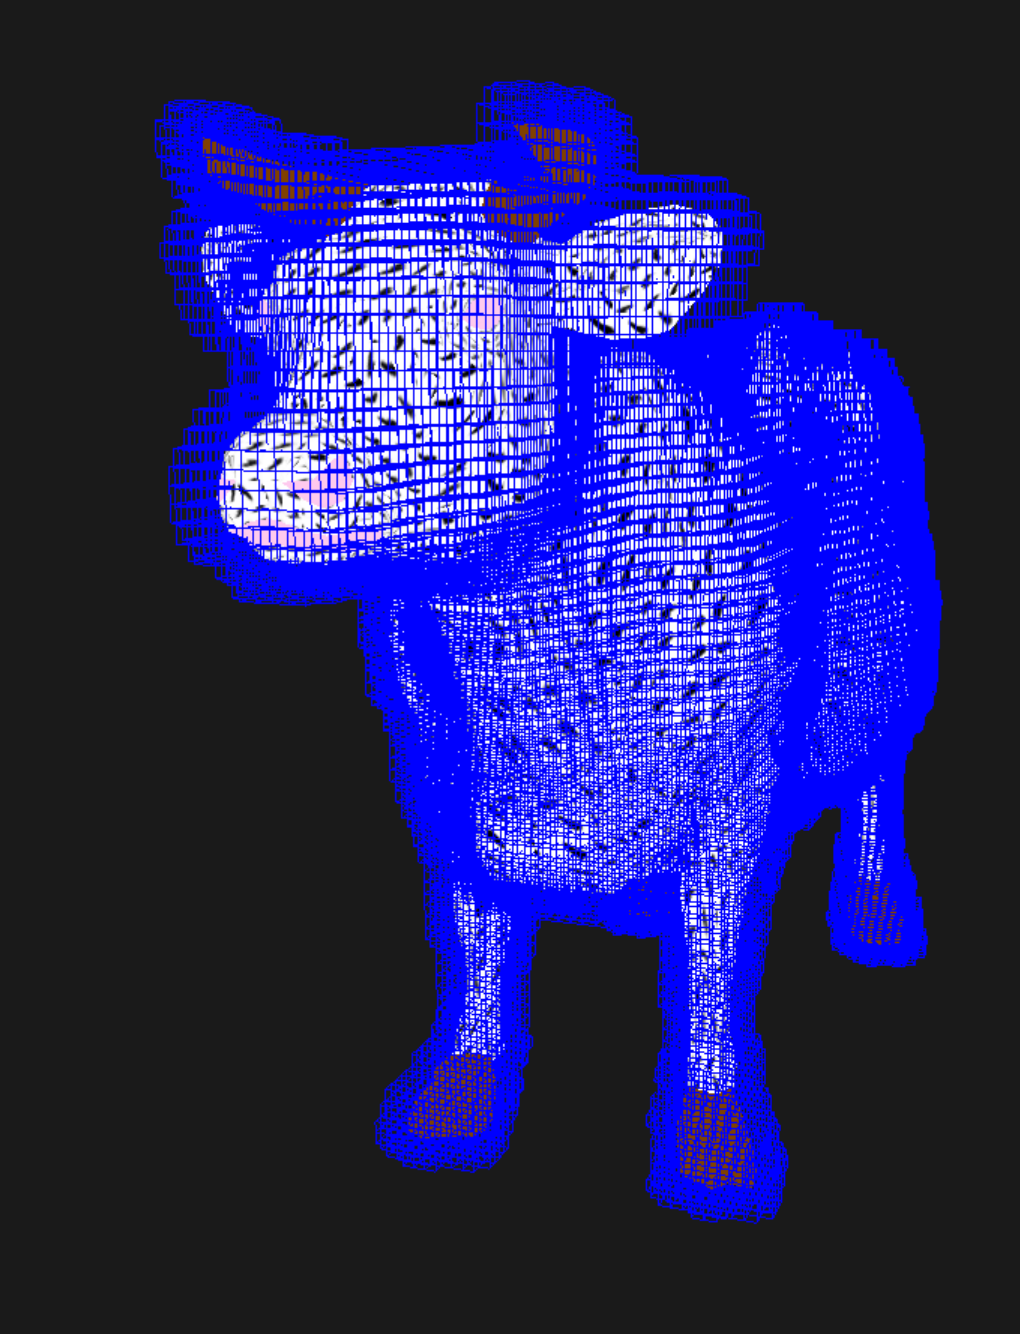
\includegraphics[width=\textwidth]{cow-octree-7.png}
        \caption{Octree nivel 7.}
    \end{subfigure}
    \caption{Distintos niveles de un octree disperso.}
    \label{fig:octree-levels}
\end{figure}

Dado que la estructura tiene como máximo $512$ o $1024$ vóxeles de resolución, sin importar la geometría de la escena, los cálculos sobre ella son independientes de la complejidad de la geometría.

\subsection{Nodos, bricks y vóxeles}\label{sec:nodes_and_bricks}

Los nodos del árbol no almacenan los vóxeles mencionados en \ref{sec:voxelization}.
Cada nodo almacena únicamente un puntero a sus, como máximo, $8$ hijos.

Cada nodo tiene asociado un \textbf{brick}, otra estructura que también representa una región del espacio.
Cada brick está dividido en 27 vóxeles, distribuidos en una estructura de $3\times3\times3$.
Son estos vóxeles los que almacenan los valores de la escena.
Los nodos solo contienen punteros a sus hijos, existen para obtener la estructura del árbol.
Los nodos proveen la estructura mientras que los bricks y vóxeles los datos.

En la figura \ref{fig:node_and_brick} se puede observar un nodo con su brick asociado de la manera en la que se disponen en el espacio.
Los bricks ocupan más espacio que sus nodos, ya que los vóxeles se centran en los vértices del nodo.
Esto es necesario para que los bricks información con bricks de nodos vecinos, lo que garantiza que la interpolación dentro de un solo nodo tome en cuenta los valores de sus vecinos.
Colocar los vóxeles en las esquinas de los nodos genera una frontera compartida entre bricks de nodos vecinos, como se puede ver en la figura \ref{fig:brick_border_overlap}.
La frontera entre dos nodos adyacentes del mismo nivel son los 9 vóxeles de la cara compartida entre los nodos, 3 en el caso 2D apreciable en las figuras, que están presentes en los bricks de ambos nodos. 
Como consecuencia, la estructura tiene información repetida, necesario para que funcione la interpolación cuando se quiera generar la imagen final.
Un \textit{shader} llamado \textit{border\_transfer}, es el que se encarga de lograr la coherencia en la frontera entre dos \textit{bricks}.
Se explicará en la Sección \ref{sec:border_transfer}.

\begin{figure}[h!]
    \centering
    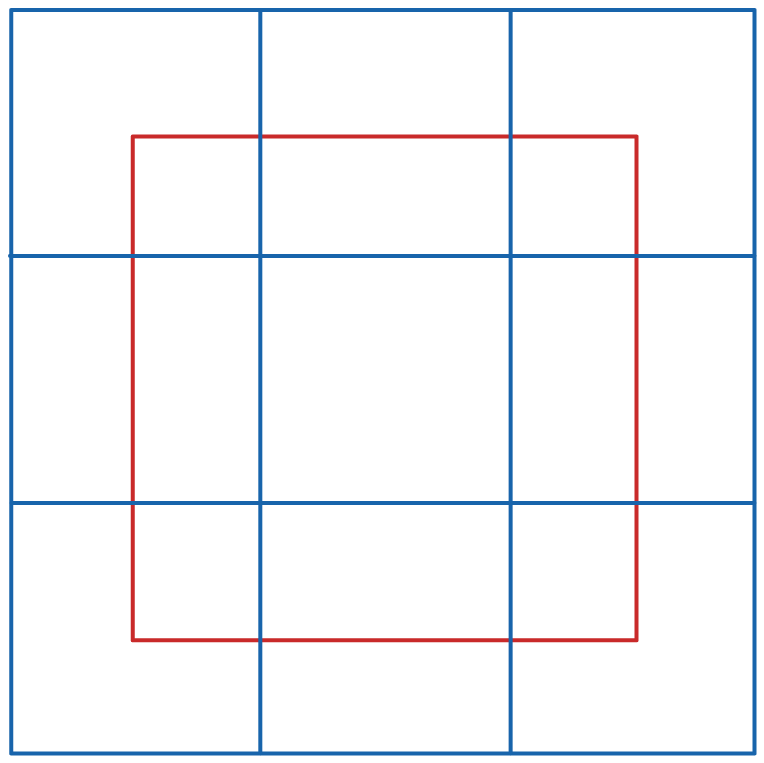
\includegraphics[width=.3\textwidth]{node-and-brick.png}
    \caption{Nodo (en rojo) con su brick asociado (azul).}
    \label{fig:node_and_brick}
\end{figure}

\begin{figure}[h!]
    \centering
    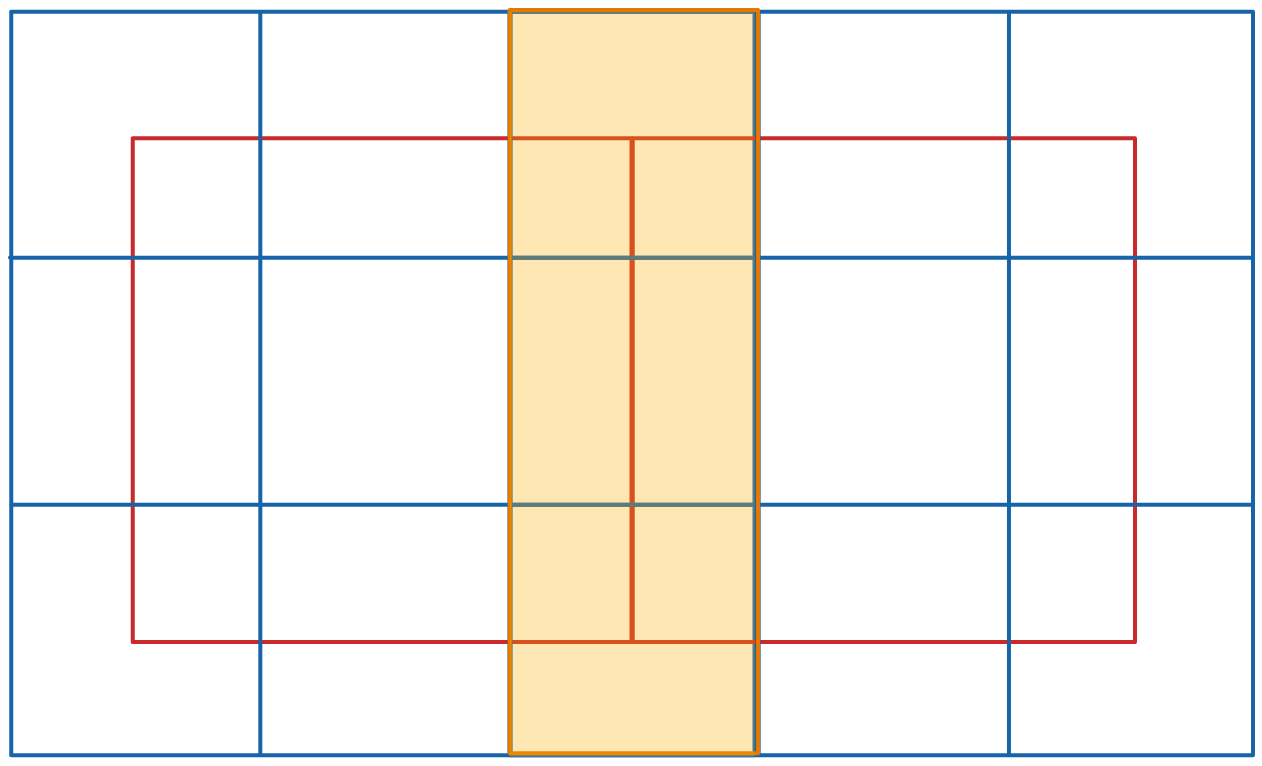
\includegraphics[width=.5\textwidth]{brick-border-overlap.png}
    \caption{Solapamiento entre vóxeles de bricks de nodos vecinos.}
    \label{fig:brick_border_overlap}
\end{figure}

\subsection{Construcción}\label{design:svo_construction}

Para generar el octree disperso se usa la lista de vóxeles generada durante la voxelización.
Se empieza con un árbol con un solo nivel, con un solo nodo que representa toda la escena.
Empezando en el primer nivel del árbol y descendiendo a lo largo de los niveles, se subdividen los nodos que contienen geometría.
Un nodo debe ser subdividido cuando existe un vóxel en la lista con coordenadas dentro del nodo y no se llegó a un cierto nivel deseado.
El algoritmo utilizado se detalla a continuación.

Dado un nivel $i$ del árbol, dos programas principales son ejecutados en secuencia para generar el nivel $i + 1$: \textit{flag\_nodes} y \textit{allocate\_nodes}.

Se corre un hilo de \textit{flag\_nodes} por cada vóxel de la lista de vóxeles.
Dado un vóxel, se recorre el árbol, hasta llegar a $i$, el último nivel creado hasta el momento.
Para recorrer el árbol, cada hilo comienza en su primer nodo.
Al llegar a un nodo en el nivel $i$, se marca uno de los $8$ punteros a sus hijos.
Cada hijo del nodo representa un octante en el espacio dentro de él.
Se usa la posición del vóxel para determinar a qué octante pertenece, el puntero a este hijo es marcado.

Realizar esta marca es un proceso idempotente, ya que se limita a cambiar el bit mas significativo del puntero a 1.
Es idempotente porque el resultado de la operación es el mismo sin importar la cantidad de hilos que lo realicen.

Luego, se ejecuta \textit{allocate\_nodes}, que busca en el nivel $i$ los punteros marcados. 
Se corre un hilo por cada posible nodo hijo que puede ser creado en esta etapa, $8$ por cada nodo del nivel $i$.
A cada hilo se le asigna uno de los punteros de los nodos del nivel, confirma si fue marcado en el paso anterior, elimina la marca, crea el nodo hijo y agrega al puntero el indice del hijo recien creado.
El índice del nuevo hijo se crea usando un contador que es posteriormente incrementado.
Para el incremento, se usa una operación atómica que permite que dos hilos puedan crear un nodo concurrentemente sin colisión de índices.
Siempre y cuando haya geometría en la región de la escena representada por un nodo, el mismo será subdividido nivel tras nivel hasta el máximo determinado por la resolución de la grilla de vóxeles.

Esta separación entre marcar y subdividir es necesaria para prevenir problemas de concurrencia, al ser esto ejecutado en múltiples hilos.
Durante la construcción de un nivel interno del \textit{octree}, es probable que muchos hilos marquen la creación de un mismo nodo hijo.
Si el mismo hilo que se encarga de crear la marca, también crease el nodo, se tendrian nodos duplicados perdidos dentro de la memoria.
En lugar de lidiar con que todos esos hilos intenten subdividirlo, se limitan a marcarlo de manera idempotente, evitando así utilizar locks entre hilos.
Correr un solo hilo para cada posible hijo que se debe crear asegura que no se creen nodos duplicados, resolviendo así el problema de concurrencia.

Un paso de este algoritmo se puede observar en la figura \ref{fig:flag-and-allocate}.
Corriendo el algoritmo para un vóxel $x$, este debe ser ubicado en el último nivel, en el nodo punteado.
El nodo inmediatamente anterior se marca para subdividir y luego se subdivide.

\begin{figure}[ht]
    \begin{subfigure}{.32\textwidth}
        \centering
        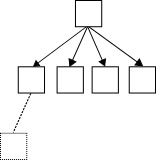
\includegraphics[width=.75\textwidth]{flag-and-allocate-start.png}
        \caption{El vóxel debe ir en el nodo punteado.}
    \end{subfigure}
    \begin{subfigure}{.32\textwidth}
        \centering
        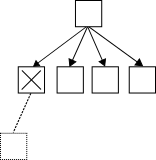
\includegraphics[width=.75\textwidth]{flag-and-allocate-flag.png}
        \caption{El nodo padre es marcado para ser subdividido.}
    \end{subfigure}
    \begin{subfigure}{.32\textwidth}
        \centering
        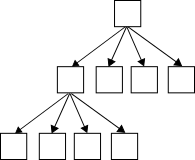
\includegraphics[width=\textwidth]{flag-and-allocate-allocate.png}
        \caption{El nodo marcado es subdividido.}
    \end{subfigure}
    \caption{Un paso del algoritmo de \textit{flag} y \textit{allocate}.}
    \label{fig:flag-and-allocate}
\end{figure}

Una vez alcanzado el último nivel, se escriben los atributos de los vóxeles en los bricks de las hojas del árbol, promediando cuando más de un vóxel tiene la misma posición en la grilla de vóxeles.
Mientras más triángulos tenga la escena original y menos resolución la grilla de vóxeles, más ocurre lo anteriormente mencionado.
% Dar la definicion de hoja aca me parece raro

% Esto creo que deberia ir en implementacion
En \ref{sec:nodes_and_bricks}, se vió como los \textit{bricks} ocupan una región más amplia del espacio que su nodo correspondiente.
Además los vóxeles conseguidos en la voxelización no estan alineados con los vóxeles de los bricks.
En la primer parte de la figura \ref{fig:voxels-to-bricks} se puede observar un brick, cuyos vóxeles estan numerados, solapado con 4 vóxeles generados en el paso de voxelización, cada uno con su color.
En el espacio de la escena estos coinciden con el nodo del brick, ya que la grilla utilizada para la voxelización es la misma que la determinada por los nodos del nivel mas bajo, pero llegando a un nivel mayor de resolución.
Por lo que a cada nodo le corresponden a lo sumo 8 vóxeles del paso de voxelización, si consideramos que triangulos que se solapan en un vóxel de la grilla devuelven un unico vóxel con el promedio de sus colores.

\begin{figure}[ht]
    \begin{subfigure}{.49\textwidth}
        \centering
        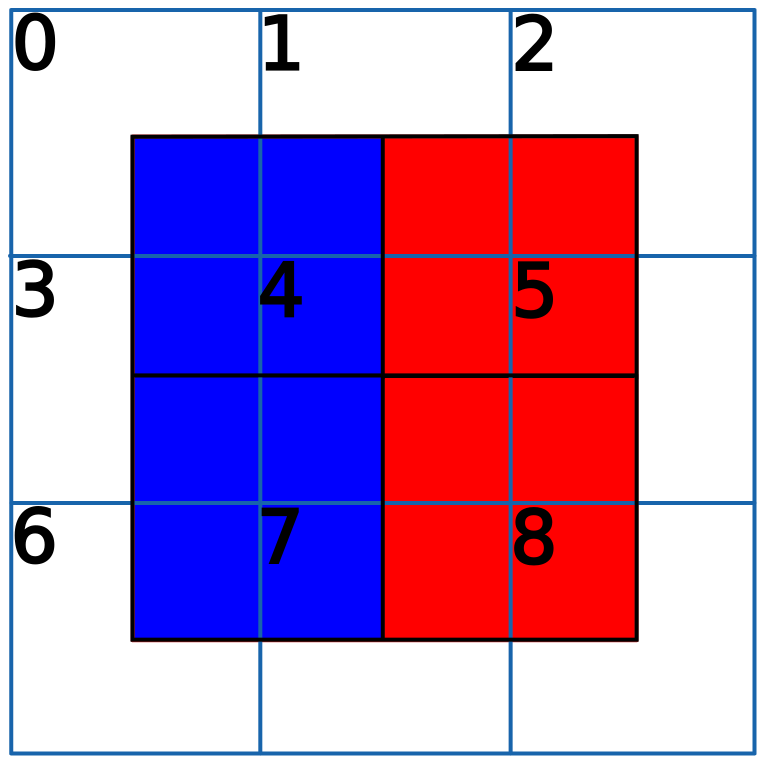
\includegraphics[width=.5\textwidth]{voxels-to-bricks.png}
        \caption{Solapamiento en el espacio de la escena entre el brick y los vóxeles.}
    \end{subfigure}
    \begin{subfigure}{.49\textwidth}
        \centering
        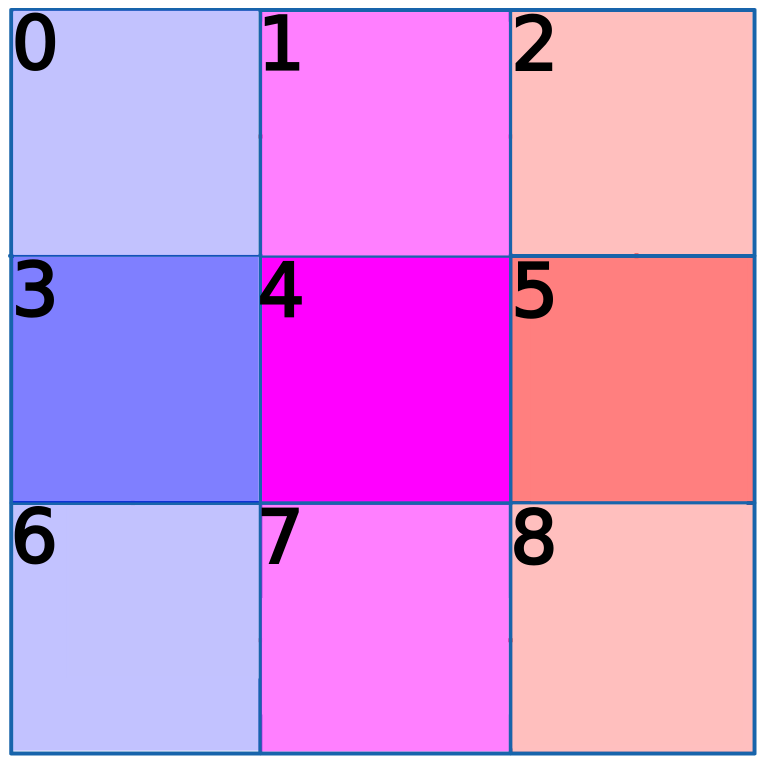
\includegraphics[width=.5\textwidth]{voxels-to-bricks-b.png}
        \caption{Brick con el valor de los vóxeles almacenados.}
    \end{subfigure}
    \caption{Vóxeles de la voxelización y su asignación a un brick.}
    \label{fig:voxels-to-bricks}
\end{figure}

Para la versión 2D a cada nodo le corresponden a lo sumo 4 vóxeles del paso de voxelización.
Se le asignan valores a todos los vóxeles del brick, utilizando la figura \ref{fig:voxels-to-bricks} como ejemplo, como se detalla a continuación:
\begin{itemize}
    \item El vóxel 4 almacena el promedio de azul y rojo
    \item El vóxel del medio de cada arista almacena el promedio de los 2 valores que le corresponden y espacio vacio, siendo el vóxel 3 un azul semi transparente con una opacidad de 0.5
    \item El vóxel de cada esquina almacena tres cuartas partes de espacio vacío, y el color correspondiente, siendo el vóxel 2 de color rojo con una opacidad de 0.25
\end{itemize}

Como resultado, se esparcen los valores de los vóxeles del paso de voxelización a los vóxeles del \textit{brick}.
De esta figura también se desprende la necesidad del border transfer \ref{sec:border_transfer}, ya que los espacios vacios de los vóxeles del brick deben ser rellenados con información de nodos vecinos, aunque de forma transitória afectan la opacidad del vóxel.
Lo anteriormente descrito es el algoritmo que expande los vóxeles para poder llenar las $3\times3\times3$ subdivisiones del \textit{brick} .
A partir de aquí, el termino ``vóxel'' refiere a una de las $27$ subdivisiones de un \textit{brick}, dado que ya se procesó la lista generada durante la voxelización.

\subsection{Border transfer}\label{sec:border_transfer}

Como se mostro en la figura \ref{fig:brick_border_overlap}, los vóxeles frontera entre \textit{bricks} adyacentes corresponden al mismo espacio en la escena.
Sin embargo, cada nodo tiene su propio \textit{brick}, pero esos \textit{bricks} no comparten memoria entre ellos, habiendo así vóxeles que pertenecen a \textit{bricks} diferentes pero corresponden al mismo espacio en la escena.
Es necesario asegurarse que los valores almacenados en esos vóxeles frontera tengan el mismo valor para asegurar coherencia y una correcta interpolación a la hora de generar la imagen final.
Sin embargo, luego de aplicar \textit{spread\_leaves}, los vóxeles frontera pueden tener valores distintos entre \textit{bricks} vecinos.
Para igualarlos, se promedian los valores de la frontera con la del \textit{brick} vecino.
Además este paso es necesario para rellenar los espacios vacios vistos en la sección anterior.

El shader \textit{border\_transfer} se encarga de promediar los valores en la frontera de cada \textit{brick} con la de sus vecinos, en los ejes X, Y y Z.
De esta manera, aún cuando un vóxel puede estar en varios \textit{bricks}, en $8$ como máximo para los vóxeles en las esquinas de los \textit{bricks}, su valor va a ser siempre el mismo en cada uno de ellos. % Creo que tiene razon Eduardo, pero no hay ganas de cambiarlo
En la figura \ref{fig:border_transfer} se puede apreciar este proceso, realizado para el eje X, entre dos \textit{bricks} vecinos con los vóxels que comparten enmarcados.

\begin{figure}[h!]
    \centering
    \begin{subfigure}{1.0\textwidth}
        \centering
        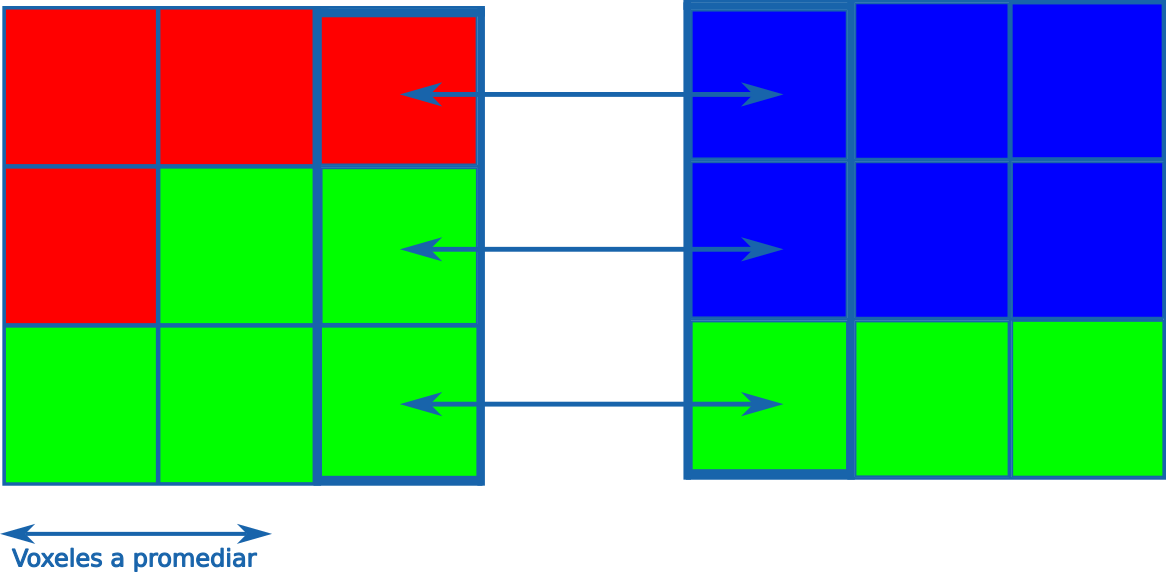
\includegraphics[width=1.0\textwidth]{border-transfer.png}
        \caption{\textit{Bricks} vecinos antes del border transfer.}
    \end{subfigure}
    \begin{subfigure}{1.0\textwidth}
        \centering
        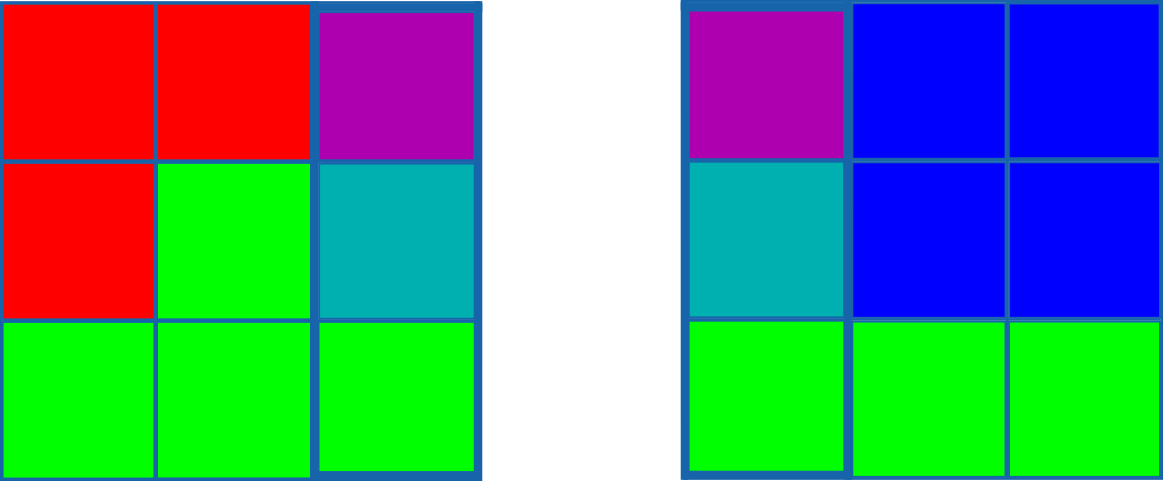
\includegraphics[width=1.0\textwidth]{border-transfer-b.png}
        \caption{\textit{Bricks} vecinos después del border transfer.}
    \end{subfigure}
    \caption{\textit{Bricks} vecinos en el \textit{eje X}.}
    \label{fig:border_transfer}
\end{figure}

\subsection{Nodos frontera}

El paso anterior tiene un problema, asume que todos los nodos tienen vecinos.
Al usar un \textit{octree} disperso, no existen nodos en donde no hay geometría.
Como se vio en la sección \ref{sec:border_transfer}, para mantener coherencia dentro de la estructura todo par de bricks vecinos deben tener valores iguales en sus vóxeles frontera.
En el límite entre la geometría y el espacio vacío existen nodos sin vecinos.
Estos nodos presentan un problema que impide una correcta interpolación, dado que no se puede promediar el valor de sus vóxeles con su vecino.
Para una correcta interpolación, es necesaria una capa de nodos extra, los que llamaremos \textbf{nodos frontera}, que representa el espacio vacío adyacente a la geometría.

Los nodos frontera se añaden en cada nivel del árbol a la hora de construírlo.
Sus \textit{bricks} en principio no contienen valores, existen para asegurar una correcta interpolación en los extremos de la geometría.
Se realiza un border transfer extra entre los nodos frontera y sus vecinos, de manera que los vóxeles compartidos entre los dos tengan el mismo valor.
El mismo problema no se vuelve a generar entre estos nodos frontera y el espacio vacío, dado que los vóxeles compartidos entre ellos tienen opacidad nula.
El resultado de la introducción de los nodos frontera se observa en la figura \ref{fig:nodos_frontera}.

En el algoritmo de \textit{cone tracing}, se toma la intersección del cono con el nodo.
Luego se toma una muestra del \textit{brick}, en el lugar donde interseca con el cono.
Para mejor entender el problema solucionado por los nodos frontera, veamos un ejemplo
usando un rayo en lugar de un cono, ya que el algoritmo toma muestras en puntos especificos del nodo y usa el nivel del árbol como aproximación del cono.

\begin{figure}[h!]
    \centering
    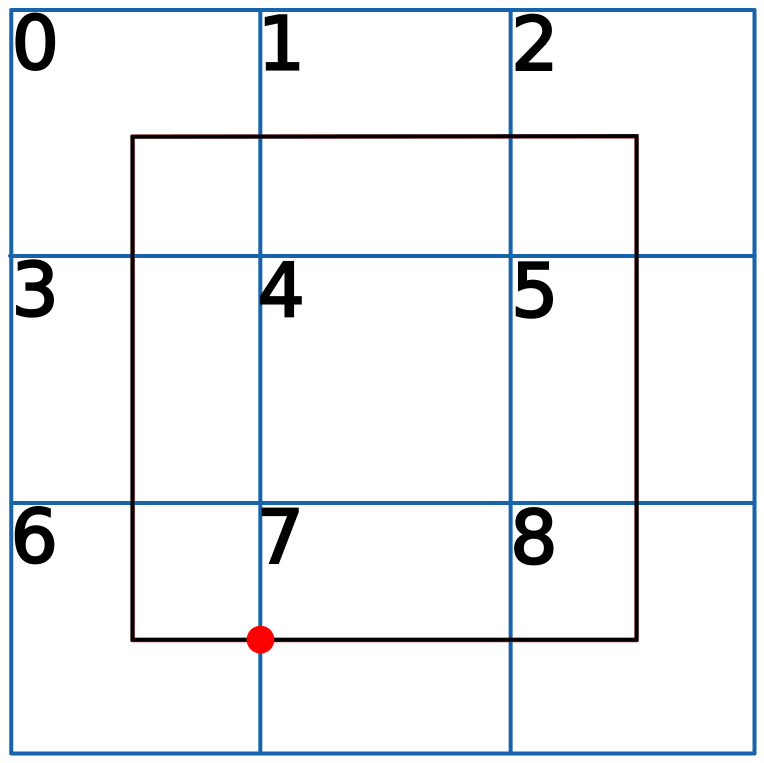
\includegraphics[width=.5\textwidth]{sampling-interpolated.png}
    \caption{Muestreo interpolado.}
    \label{fig:muestreo-interpolado}
\end{figure}

Consideremos un nodo como el de la figura \ref*{fig:muestreo-interpolado}, cuyo \textit{brick} asociado tiene sus vóxeles numerados.
Este nodo no tiene vecinos.
Digamos que su vóxel 6 es de color azul y su vóxel 7 color rojo, ambos con opacidad 1.
Si se tiene un rayo que interseca en algun punto entre ambos vóxeles, como se puede ver representado con un punto rojo en la figura \ref{fig:muestreo-interpolado}, el valor muestreado sera violeta con un mayor componente azul, la interpolación lineal entre ambos.

\begin{figure}[h!]
    \centering
    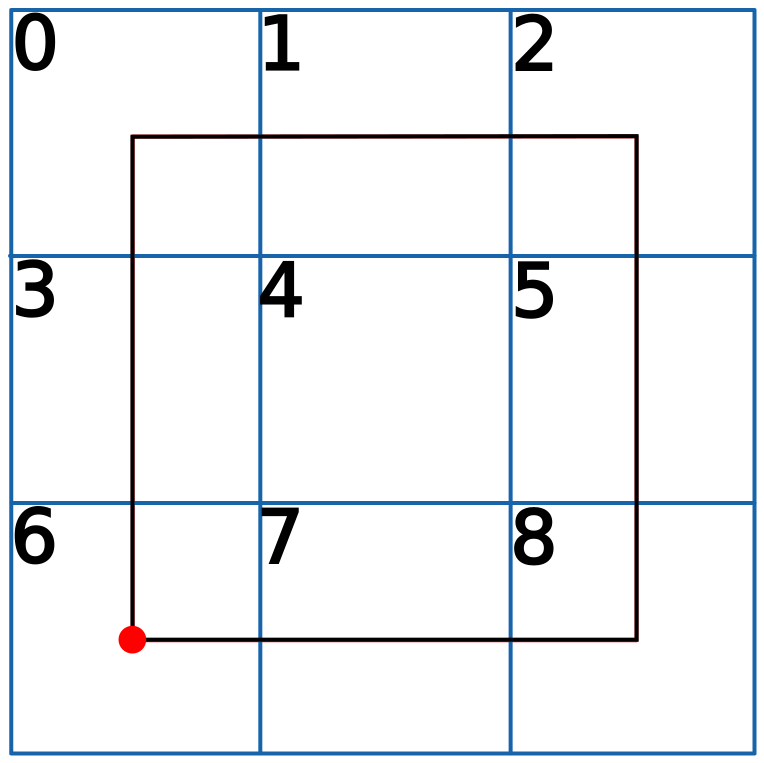
\includegraphics[width=.5\textwidth]{sampling-center-voxel.png}
    \caption{Muestreo del centro de un vóxel.}
    \label{fig:muestreo-centro-voxel}
\end{figure}

Si un rayo interseca con el centro del vóxel como en la figura \ref{fig:muestreo-centro-voxel}, el color muestreado sera azul con opacidad 1.
\begin{figure}[h!]
    \centering
    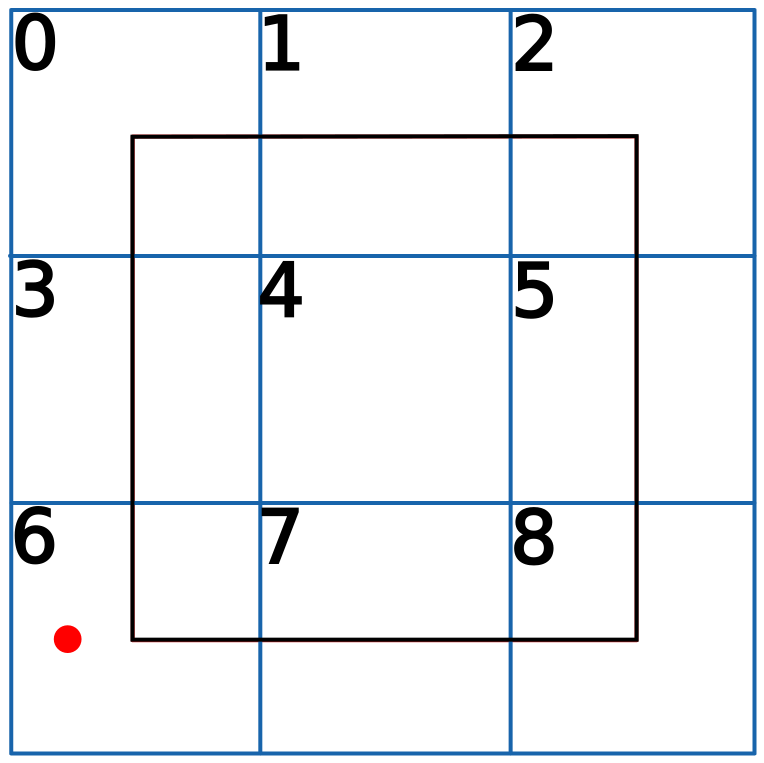
\includegraphics[width=.5\textwidth]{sampling-vacio.png}
    \caption{Muestreo con resultado vacío.}
    \label{fig:muestreo-vacio}
\end{figure}

¿Pero que ocurre cuando el rayo interseca como se ve en la figura \ref{fig:muestreo-vacio}?
Siguiendo la misma lógica, debería ser una interpolación entre azul y vacio, el cual sería azul con una opacidad menor a 1.
Sin embargo, el rayo solo puede intersecar con nodos, no \textit{bricks}, por lo que la intersección es vacia.
Pero eso es inconsistente, dado que ese vóxel tiene un valor, aunque no haya nodo ahí.
Si el nodo tuviese un vecino en X, el rayo intersecaría con el vecino, evitando el problema.
Y esa es la solución al problema, agregar uno nodo en este espacio sin geometría.

\begin{figure}[h!]
    \centering
    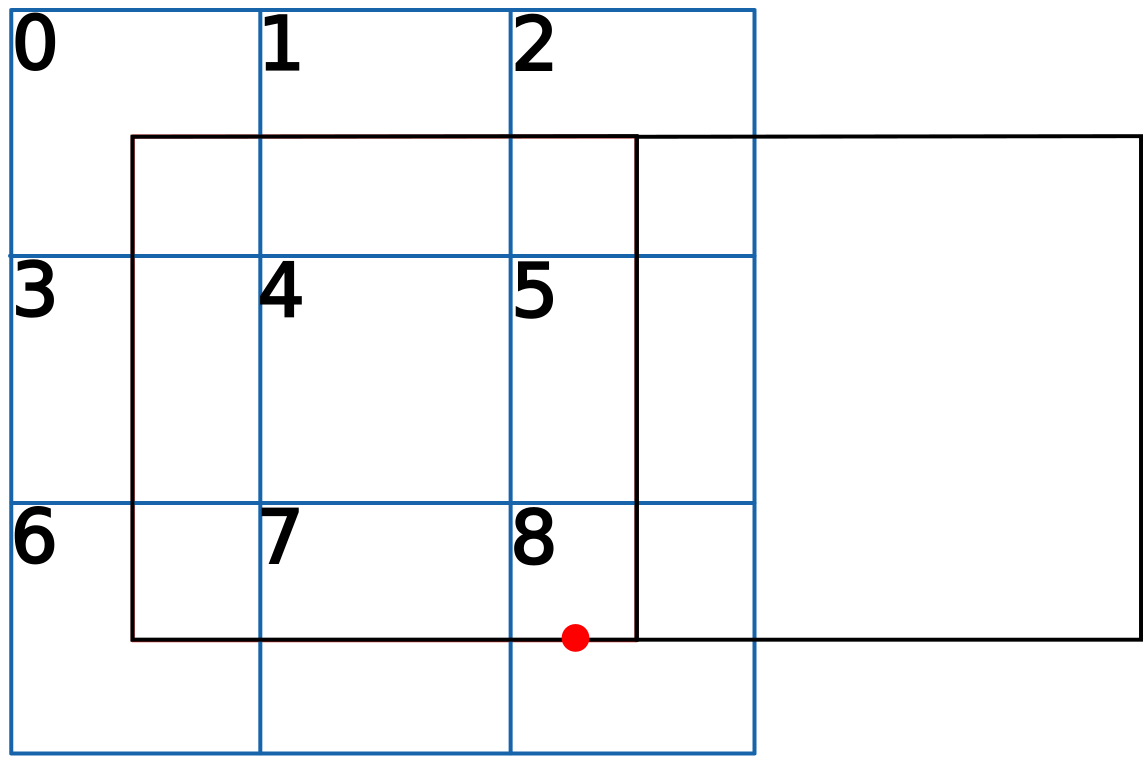
\includegraphics[width=.5\textwidth]{sampling-frontera.png}
    \caption{Muestreo con nodo frontera.}
    \label{fig:muestreo-frontera}
\end{figure}

En la figura \ref{fig:muestreo-frontera} se tiene el nodo frontera y su brick con sus vóxeles numerados, al lado del nodo original que no tenia vecinos y el mismo rayo de la figura \ref{fig:muestreo-vacio}.
El vóxel 8 va a tener color azul y opacidad 1, dado que los vóxeles compartidos entre vecinos siempre deben tener el mismo valor, y la intersección del rayo con la estructura ya no va a ser vacía llevando al resultado deseado del muestreo.

\begin{figure}
    \begin{subfigure}{.49\textwidth}
        \centering
        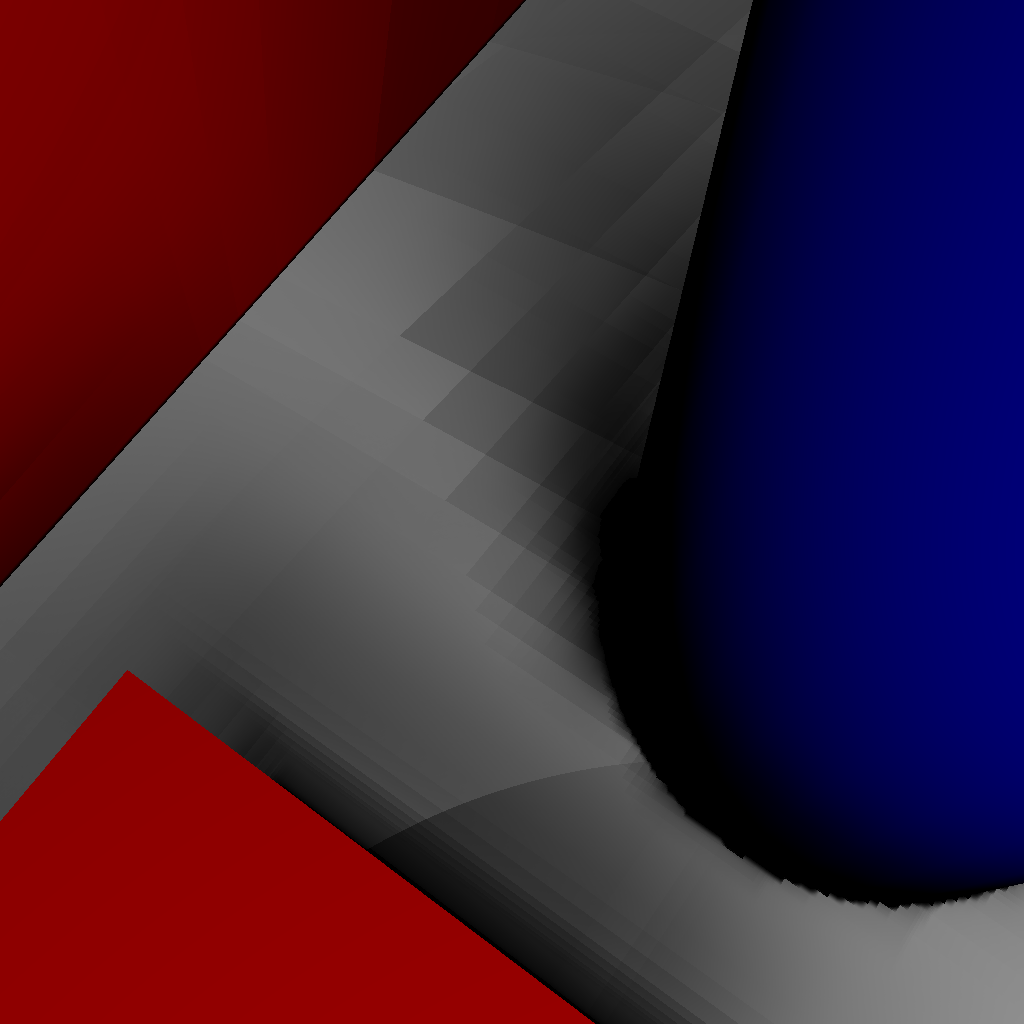
\includegraphics[width=\textwidth]{sombra-no-interpolada.png}
        \caption{Sin nodos frontera.}
    \end{subfigure}
    \begin{subfigure}{.49\textwidth}
        \centering
        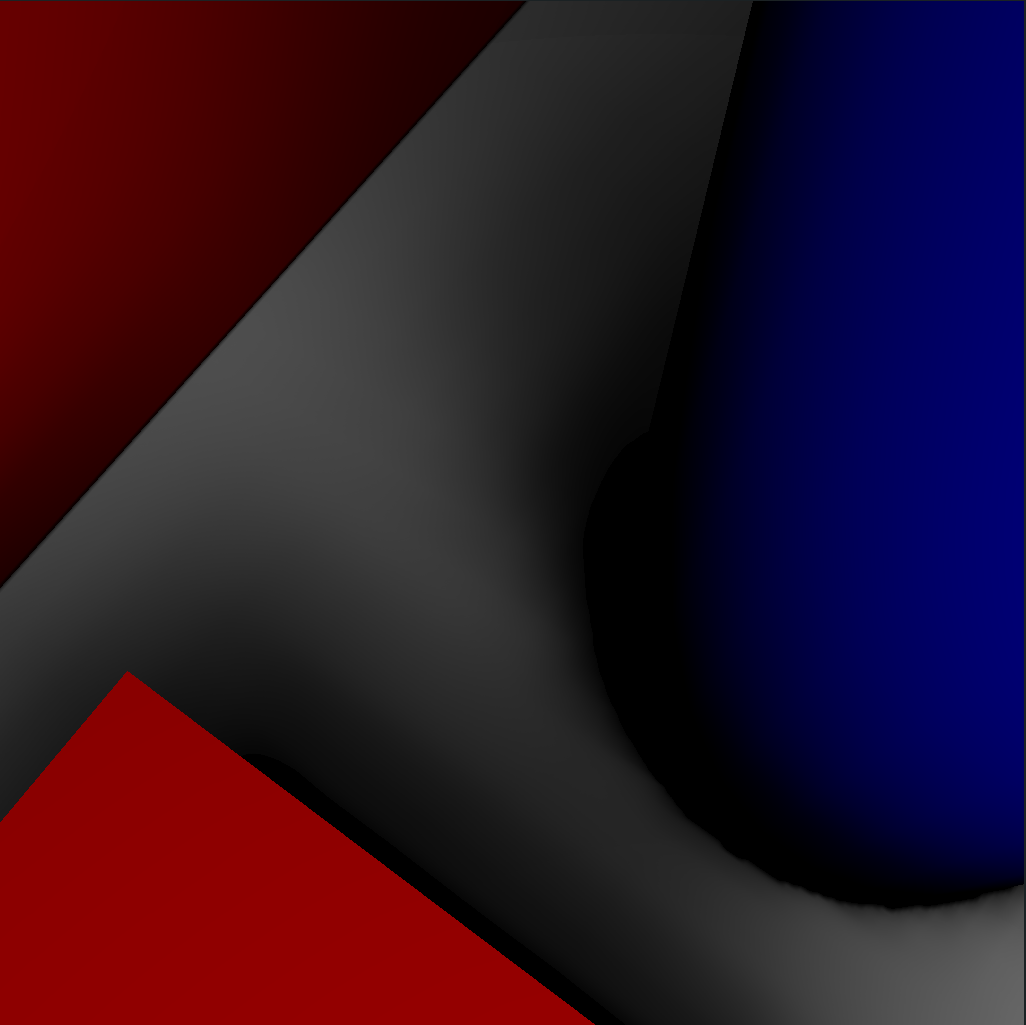
\includegraphics[width=\textwidth]{sombra-interpolada.png}
        \caption{Con nodos frontera.}
    \end{subfigure}
    \caption{Diferencia causada por nodos frontera.}
    \label{fig:nodos_frontera}
\end{figure}

\subsection{Filtrado}\label{design:filtering}

Una vez que todos los atributos se encuentran en las hojas del octree, los mismos seran filtrados a posiciones superiores.
Filtrarlos implica promediarlos de tal manera que para un nodo interior (no hoja) $A$, su brick tenga un promedio de la información contenida en los bricks de todos sus hijos.
El proceso se realiza en $n - 1$ pasos, siendo $n$ el nivel máximo del octree.
En cada paso, se calcula el valor de cada vóxel del brick del padre, usando los bricks de los hijos.

Consideremos un nodo en el penúltimo nivel, con su brick asociado y sus hijos, como muestra la figura \ref{fig:node_with_children}.
En la figuran se muestran solo $4$ hijos porque se usa como ejemplo un \textit{quadtree}, la versión 2D del \textit{octree}, ya que es mas facil de visualizar.
Cada hijo tiene a su vez su propio \textit{brick} asociado como se muestra en la figura \ref{fig:all_child_bricks}.

\begin{figure}[h!]
    \centering
    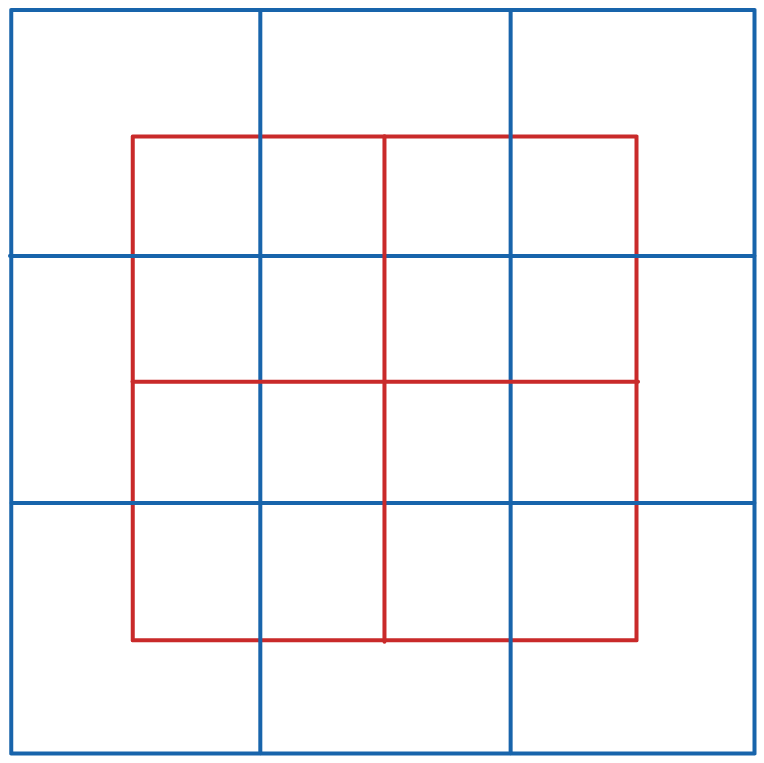
\includegraphics[width=.3\textwidth]{node-with-children.png}
    \caption{Nodo con su \textit{brick} asociado y sus hijos.}
    \label{fig:node_with_children}
\end{figure}

\begin{figure}[h!]
    \begin{center}
        \begin{subfigure}{.24\textwidth}
            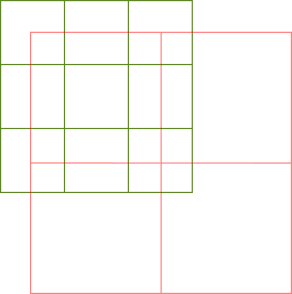
\includegraphics[width=\textwidth]{first-child-brick.png}
        \end{subfigure}
        \begin{subfigure}{.24\textwidth}
            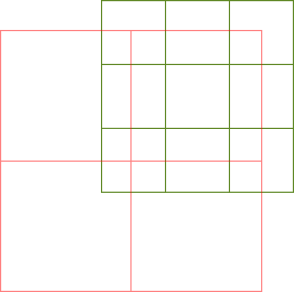
\includegraphics[width=\textwidth]{second-child-brick.png}
        \end{subfigure}
        \begin{subfigure}{.24\textwidth}
            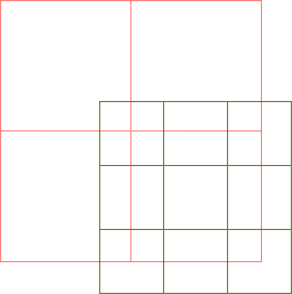
\includegraphics[width=\textwidth]{third-child-brick.png}
        \end{subfigure}
        \begin{subfigure}{.24\textwidth}
            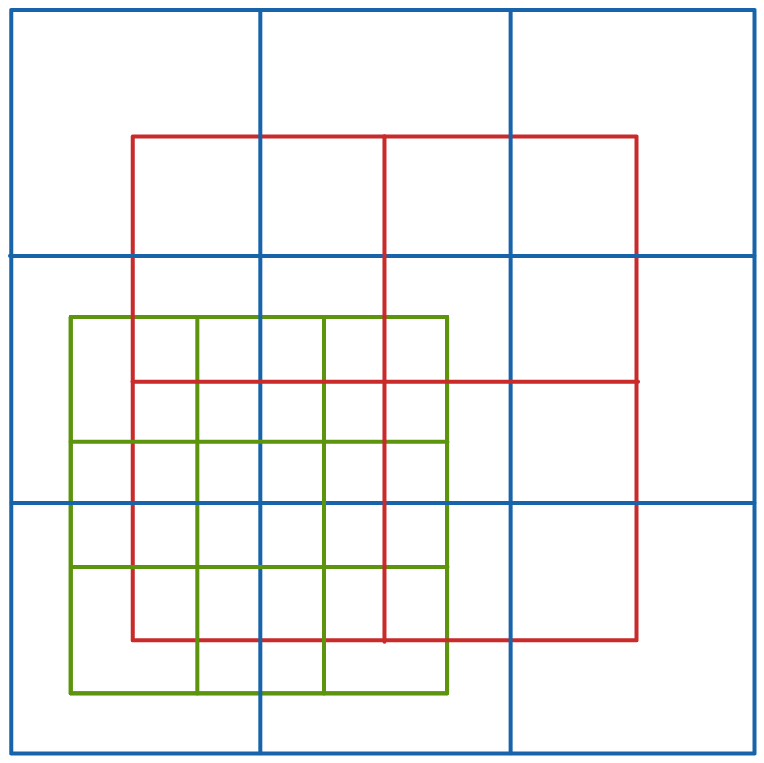
\includegraphics[width=\textwidth]{fourth-child-brick.png}
        \end{subfigure}
    \end{center}
    \caption{Bricks asociados a cada hijo del nodo.}
    \label{fig:all_child_bricks}
\end{figure}

Los valores de los vóxeles del brick padre se calculan en 4 etapas distintas, dependiendo de dónde se ubican en el \textit{brick}: Esquinas, bordes, caras, centro.
Cada una de las etapas calcula un valor parcial para un tipo de vóxel.
Es parcial porque para los vóxeles limítrofes con otro nodo, este valor tiene que luego ser agregado con el de los vecinos, con un tipo de \textit{border\_transfer}.

% El cálculo para cada etapa es el mismo para todos los vóxeles dentro de su grupo, por lo que se mostrará únicamente el calculo para un vóxel de cada grupo: esquinas, bordes, caras, y centro.
% En el caso 2D, no existe el vóxel centro.

\begin{figure}
    \centering
    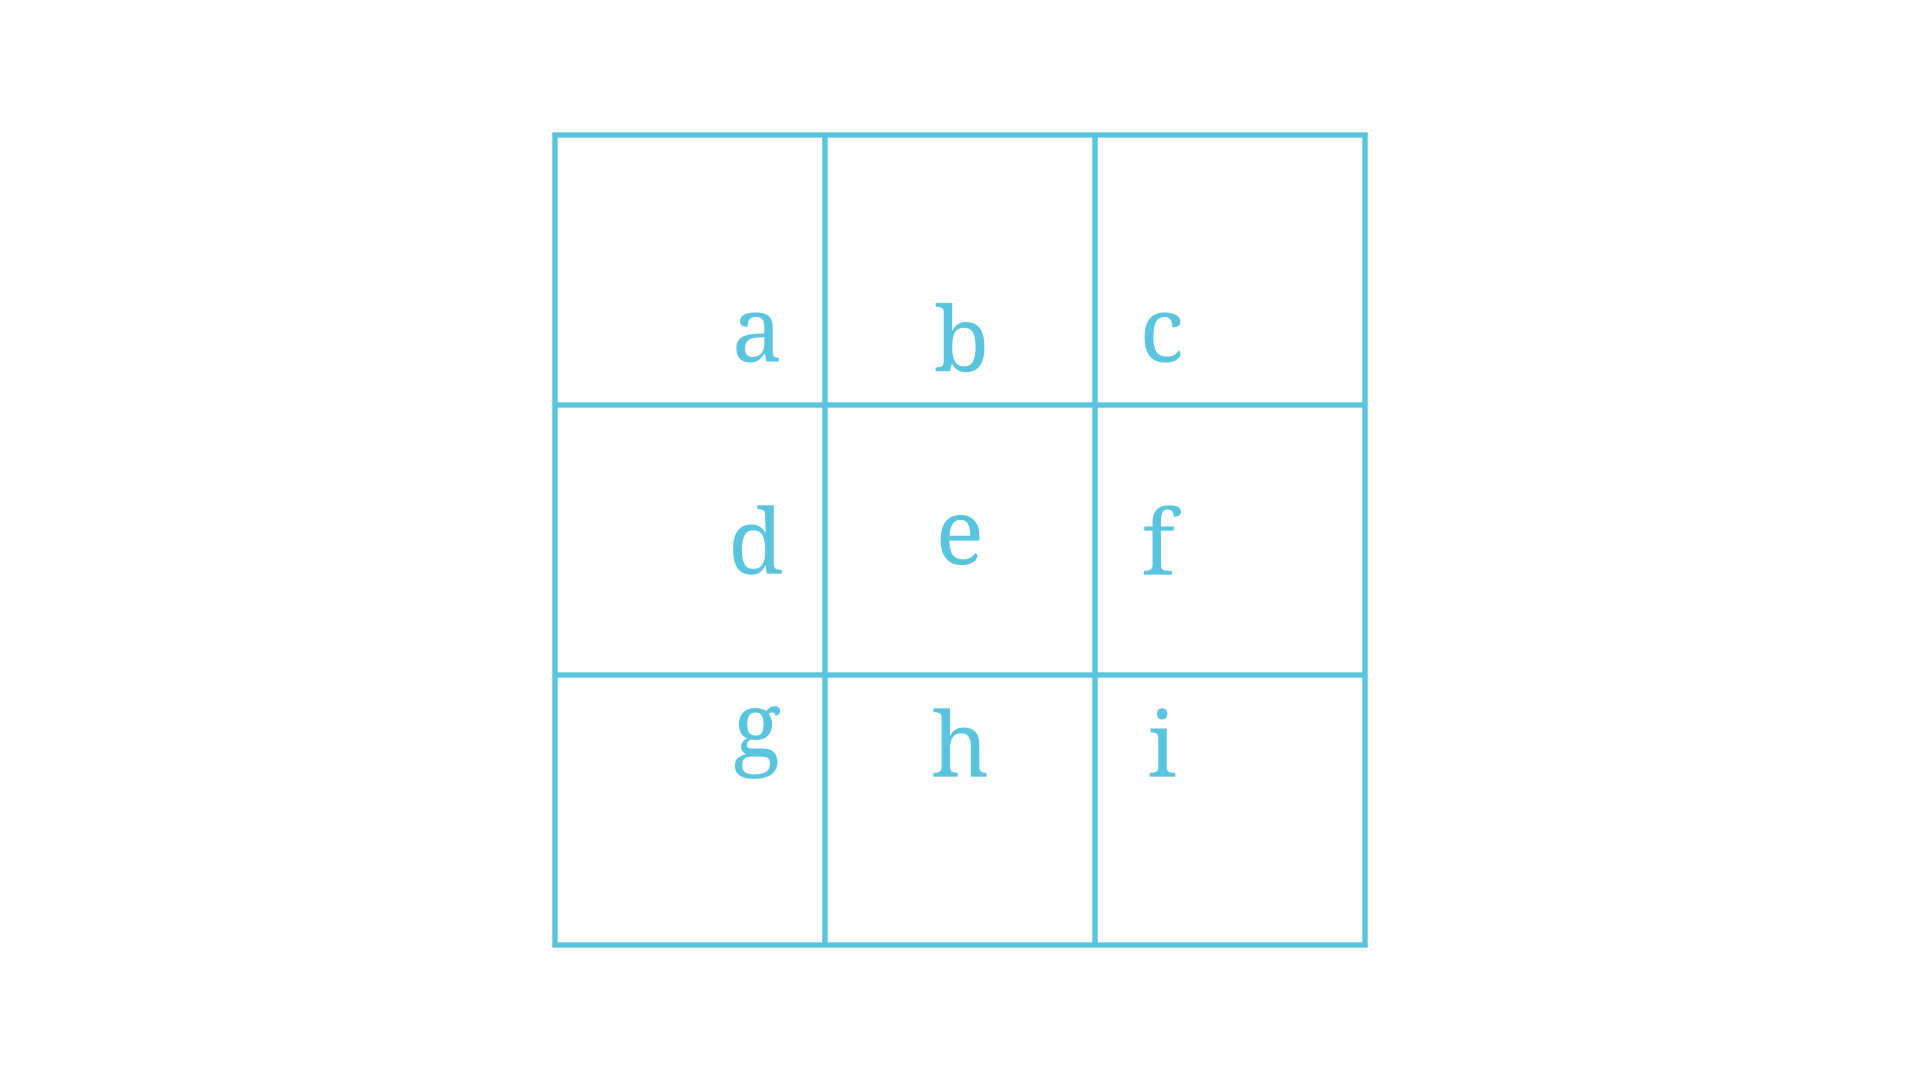
\includegraphics[width=.5\textwidth]{brick-voxel-naming.png}
    \caption{Una posible forma de referirse a cada vóxel de un brick.}
    \label{fig:brick-voxel-naming}
\end{figure}

Dado el vóxel superior izquierdo de la figura \ref{fig:svo_filtering_corners}, se considera solo el brick del hijo superior izquierdo del nodo.
De ese brick, se consideran los vóxeles amarillos en la figura.
El valor final del vóxel del padre se calcula promediando los valores de los vóxeles del hijo, pesados por el porcentaje de solapamiento.
Si nombramos los vóxeles del brick hijo $a, \cdots, i$ y los del brick padre $a', \cdots, i'$, como en la figura \ref{fig:brick-voxel-naming}, entonces el valor del vóxel del padre se calcula como:

$$
a' = a + b * \frac{1}{2} + d * \frac{1}{2} + e * \frac{1}{4}
$$

En el caso tridimensional, hay que agregar un quinto factor multiplicado por $\frac{1}{8}$.

% Esto resulta en un kernel gaussiano. % TODO: Alguna referencia sobre kernels gaussianos? Si no no lo mencionamos

\begin{figure}
    \centering
    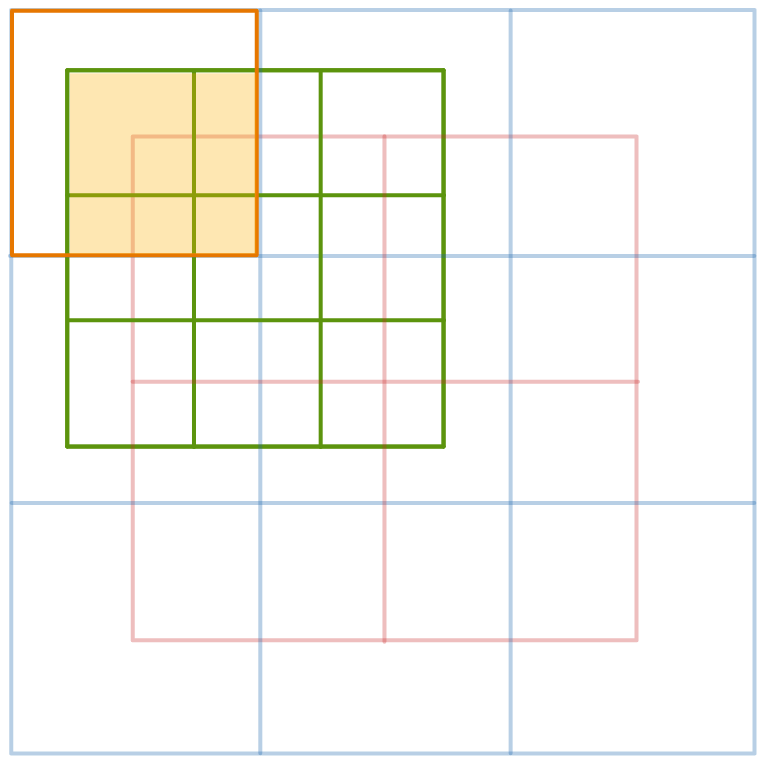
\includegraphics[width=.25\textwidth]{svo-filtering-corner.png}
    \caption{
        Filtrado para un vóxel esquina.
        Se puede ver el vóxel del brick padre cuyo valor se quiere calcular, junto con el brick del hijo y su solapamiento con este vóxel.
    }
    \label{fig:svo_filtering_corners}
\end{figure}

De la misma manera se calculan los vóxeles de los bordes y de las caras, solo que en esos casos se usan más de un brick hijo, como se puede ver en las figuras \ref{fig:svo_filtering_edges} y \ref{fig:svo_filtering_faces}.

\begin{figure}
    \begin{center}
        \begin{subfigure}{.24\textwidth}
            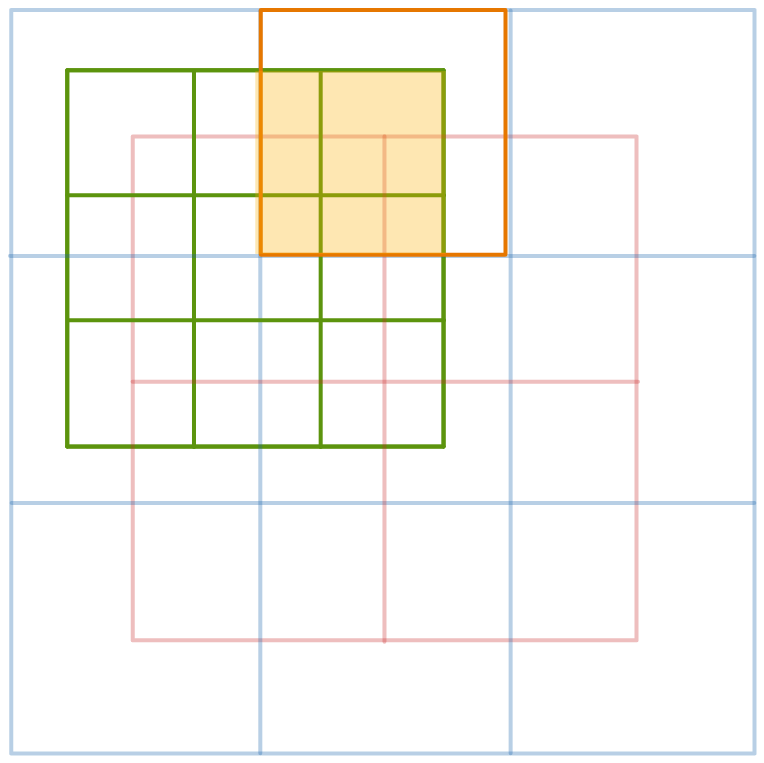
\includegraphics[width=\textwidth]{svo-filtering-edge-1.png}
        \end{subfigure}
        \begin{subfigure}{.24\textwidth}
            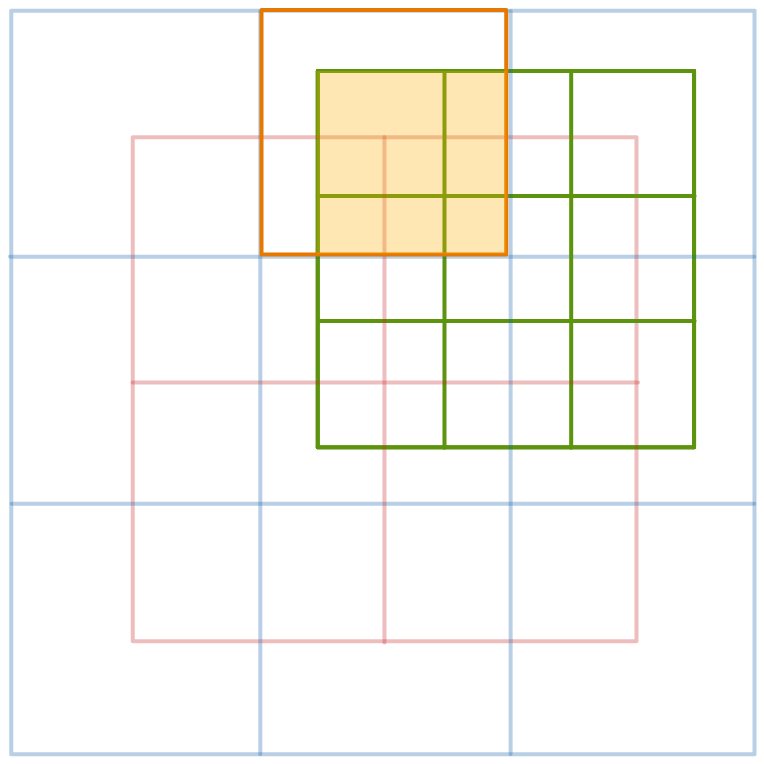
\includegraphics[width=\textwidth]{svo-filtering-edge-2.png}
        \end{subfigure}
    \end{center}
    \caption{Filtrado para un vóxel borde.}
    \label{fig:svo_filtering_edges}
\end{figure}

\begin{figure}
    \begin{center}
        \begin{subfigure}{.24\textwidth}
            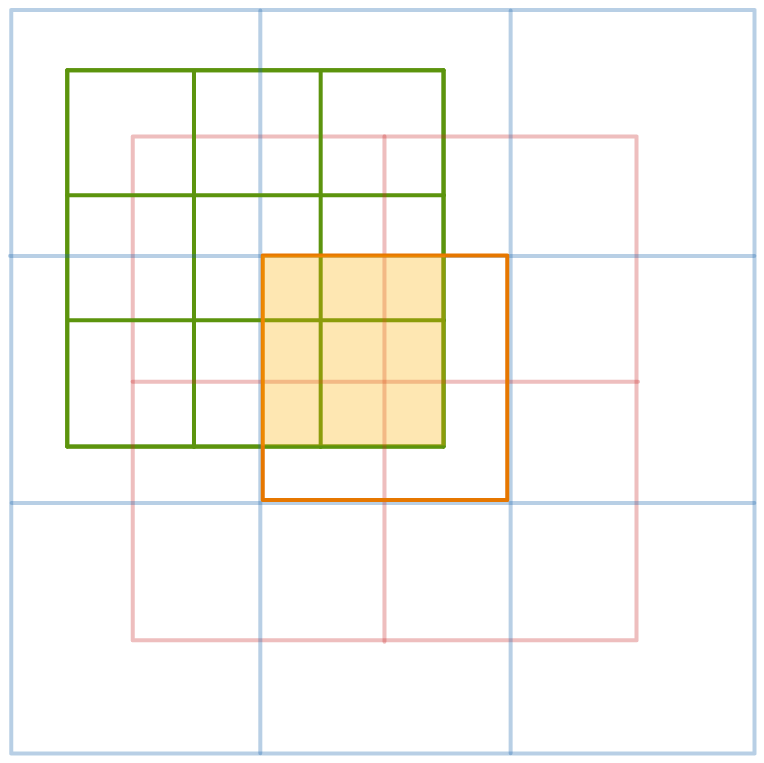
\includegraphics[width=\textwidth]{svo-filtering-face-1.png}
        \end{subfigure}
        \begin{subfigure}{.24\textwidth}
            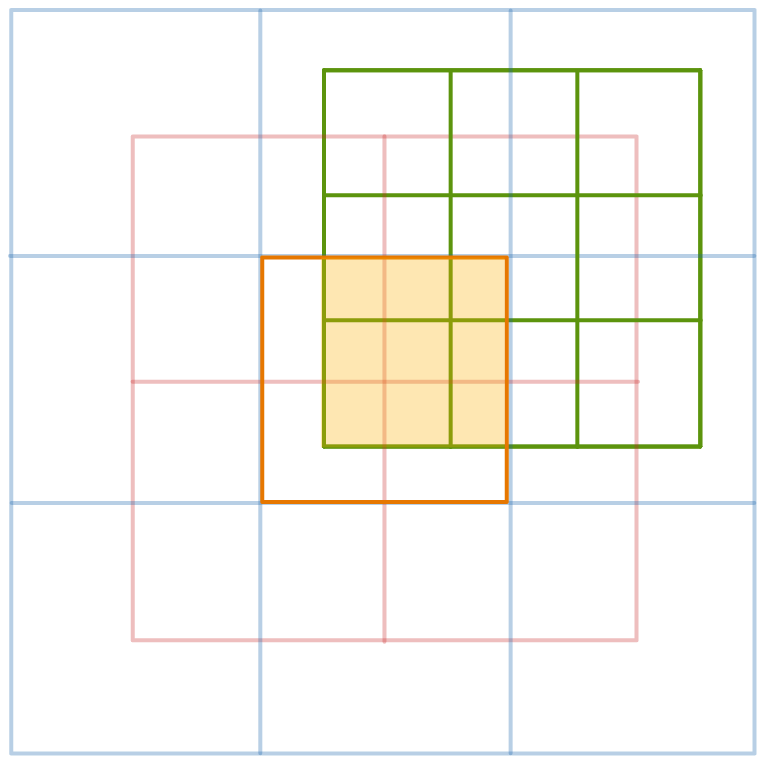
\includegraphics[width=\textwidth]{svo-filtering-face-2.png}
        \end{subfigure}
        \begin{subfigure}{.24\textwidth}
            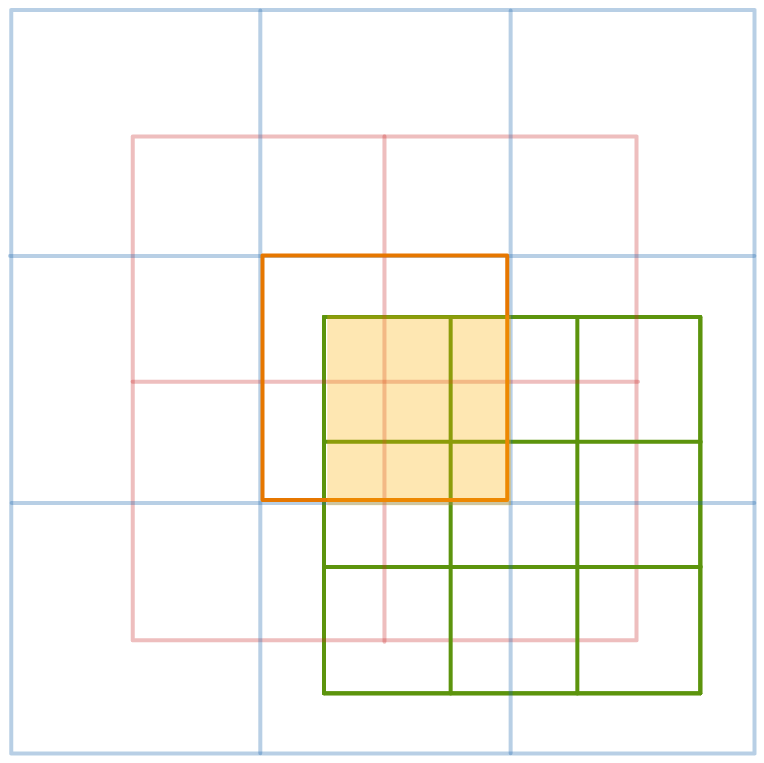
\includegraphics[width=\textwidth]{svo-filtering-face-3.png}
        \end{subfigure}
        \begin{subfigure}{.24\textwidth}
            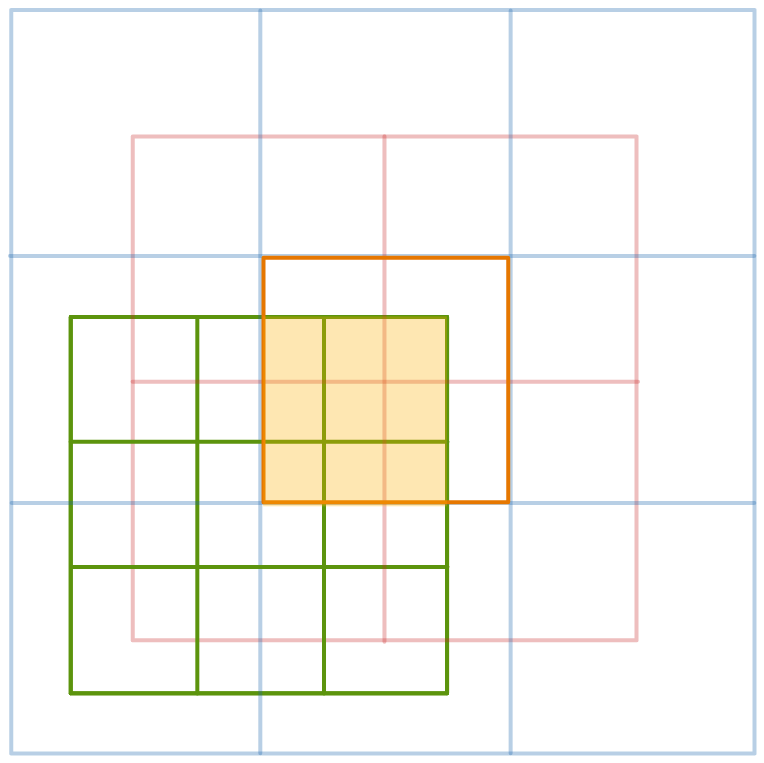
\includegraphics[width=\textwidth]{svo-filtering-face-4.png}
        \end{subfigure}
    \end{center}
    \caption{Filtrado para un vóxel cara.}
    \label{fig:svo_filtering_faces}
\end{figure}

% TODO: Solo traer de vuelta si realmente usamos normales en el código.
% Si los vóxeles almacenan normales, estas se promedian como se mencionó en la sección \ref{sec:normal_filtering}.

\subsection{Filtrado anisotrópico}

El filtrado descrito en la sección anterior resulta en vóxeles con valores independientes del punto de vista, o isotrópicos.
Una característica deseable es que los valores de oclusión y opacidad dependan del punto de vista del observador, lo que se logra en este caso guardando mas de un valor por vóxel para estas propiedades.
Es muy útil a la hora de representar un atributo en una escena 3D.

Para ilustrar el punto anterior, consideremos una escena compuesta únicamente por una pared fina.
Dado un vóxel de un nodo en un nivel alto del árbol, el nodo representa una gran región del espacio.
La región contiene únicamente una pared que pasa por su centro, y el resto de la escena es espacio vacío.
Con el filtrado presentado en las secciones anteriores, el vóxel tendrá un unico valor de opacidad que, al representar un espacio mayormente vacío, tendra un valor bajo.
Sin embargo, se observa que la percepción de la pared es muy distinta si se la ve de frente o de costado.
Como se muestra en la figura \ref{fig:anisotropic-thin-wall}, la pared vista de frente es opaca, pero vista de costado su superficie visible es practicamente nula, asemejandose a una superficie transparente.

La solución propuesta por Crassin \cite{voxel-cone-tracing} consiste en realizar el filtrado 6 veces por vóxel, uno por cada dirección alineada con los ejes: X, -X, Y, -Y, Z, -Z; y tener en cuenta la dirección a la hora de promediar los valores.
Cada uno de los 6 valores representa el vóxel visto desde una de las 6 direcciones previamente mencionadas. Por lo tanto si se observa el vóxel desde una dirección arbitraria, se calcula su oclusión y color a través de la interpolación de las tres direcciones mas cercanas.
Este tipo de filtrado se denomina \textbf{anisotrópico}, dado que depende de la dirección con que se observe al vóxel.

\begin{figure}
    \centering
    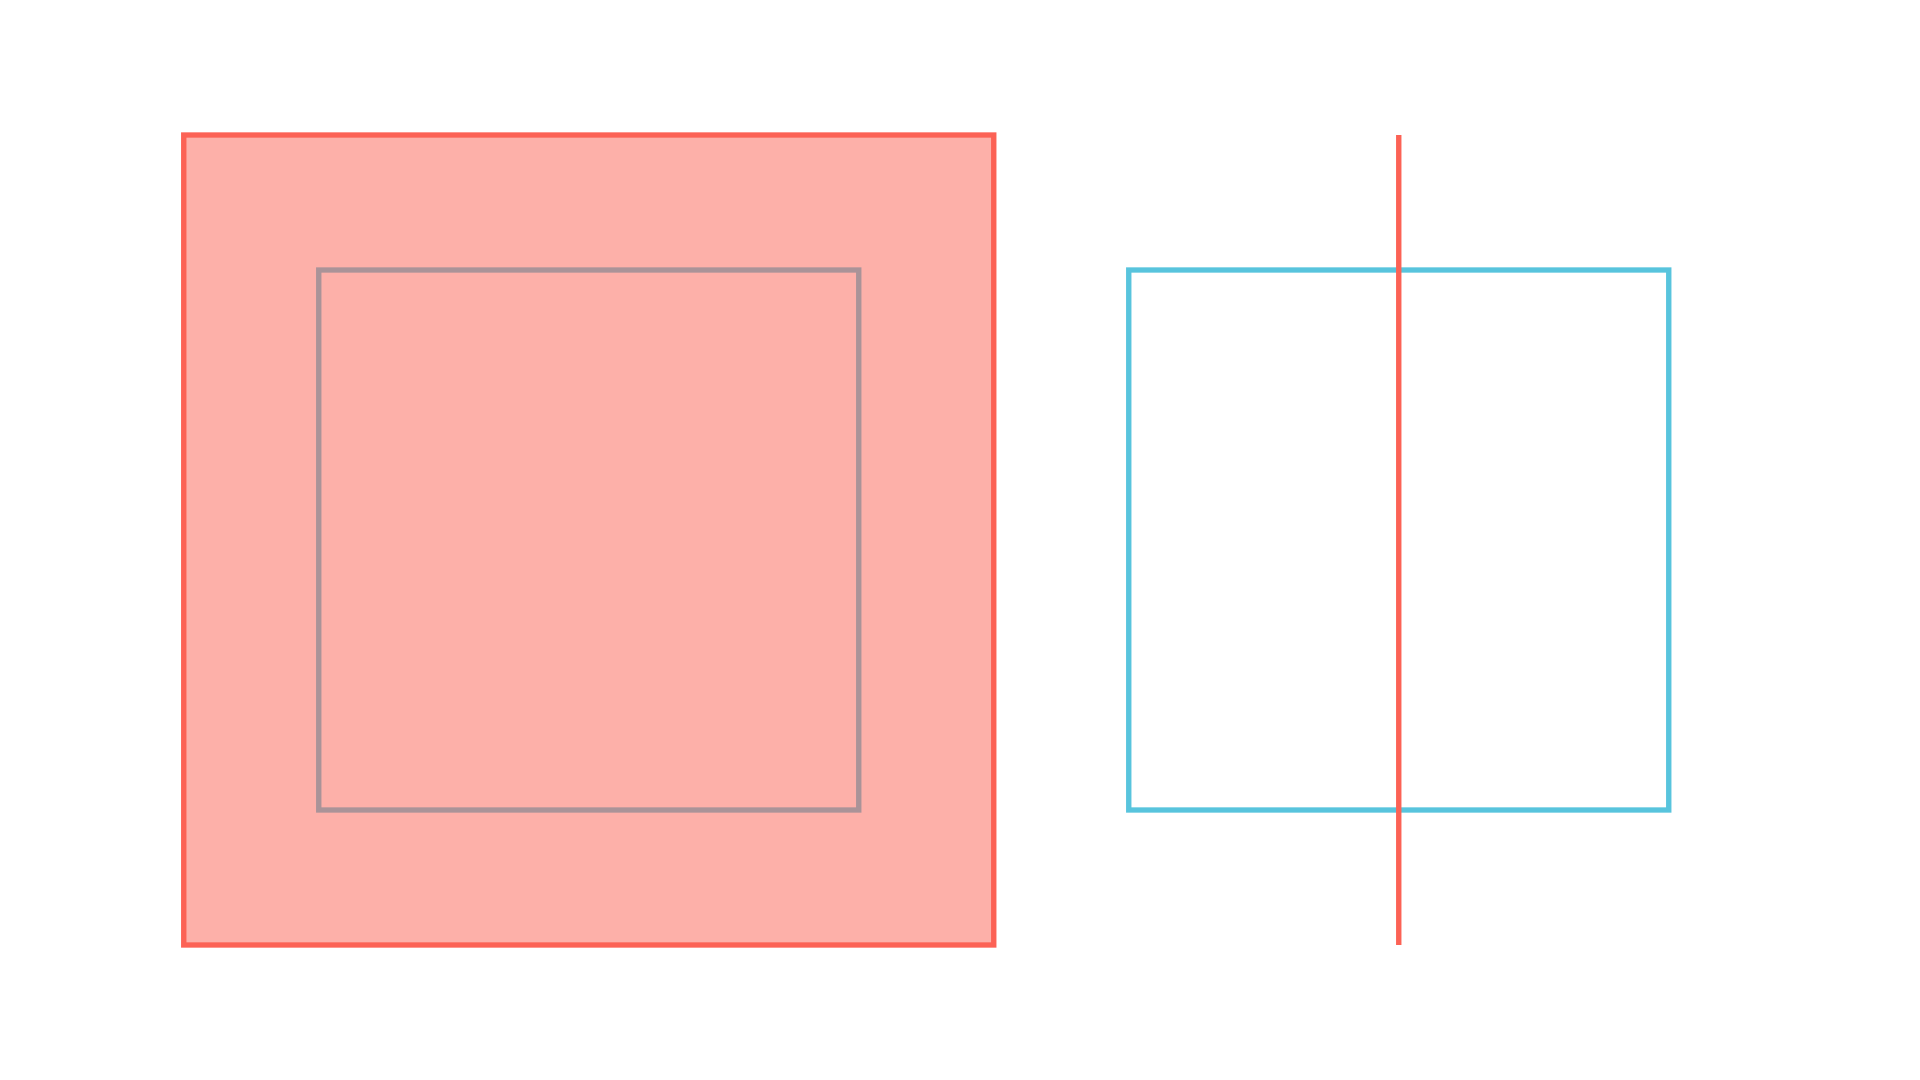
\includegraphics[width=.5\textwidth]{anisotropic-thin-wall.png}
    \caption{
        Vóxel que contiene una pared fina.
        En la izquierda, la pared se ve de frente.
        En la derecha, se ve de costado.
        Se espera que el valor del vóxel refleje esta diferencia entre las direcciones de vista.
    }
    \label{fig:anisotropic-thin-wall}
\end{figure}

Dada una dirección, por ejemplo, de izquierda a derecha, se parte de los vóxeles de la izquierda y se calcula un valor para cada fila, partiendo de estos y yendo hacia los vóxeles de la derecha.
Llamémosle al valor de cada fila \textbf{valor direccional}.
En la figura \ref{fig:svo_filtering_anisotropic} se pueden ver todos los valores direccionales que deben ser calculados para un brick en 2D, para todas las direcciones.
Para cada fila, se ejecuta un algoritmo de acumulación de opacidad que va avanzando en la dirección dada.
Si el algoritmo llega a opacidad 1, termina y devuelve el valor direccional para esa fila.

\begin{figure}
    \begin{center}
        \begin{subfigure}{.24\textwidth}
            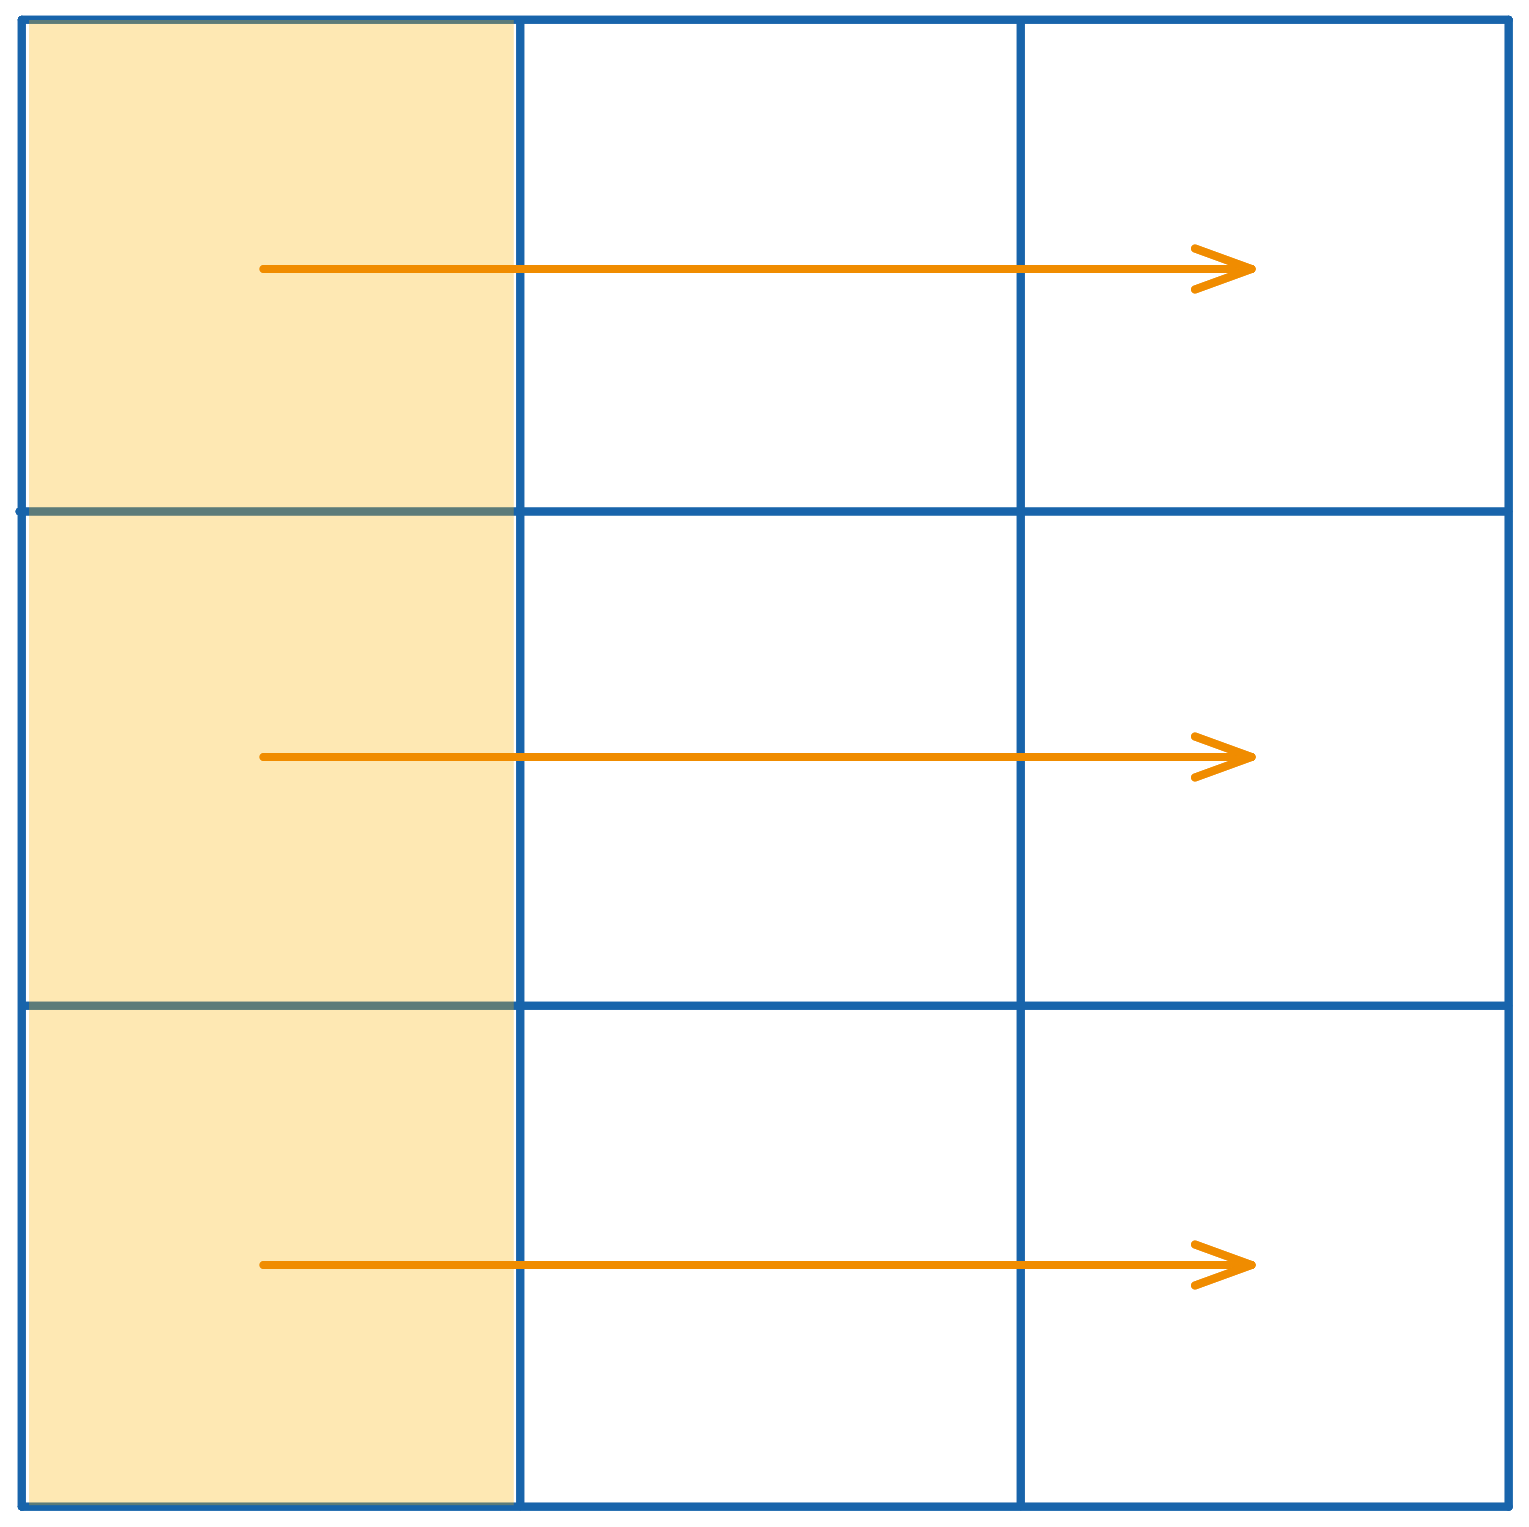
\includegraphics[width=\textwidth]{anisotropic-filtering-x.png}
        \end{subfigure}
        \begin{subfigure}{.24\textwidth}
            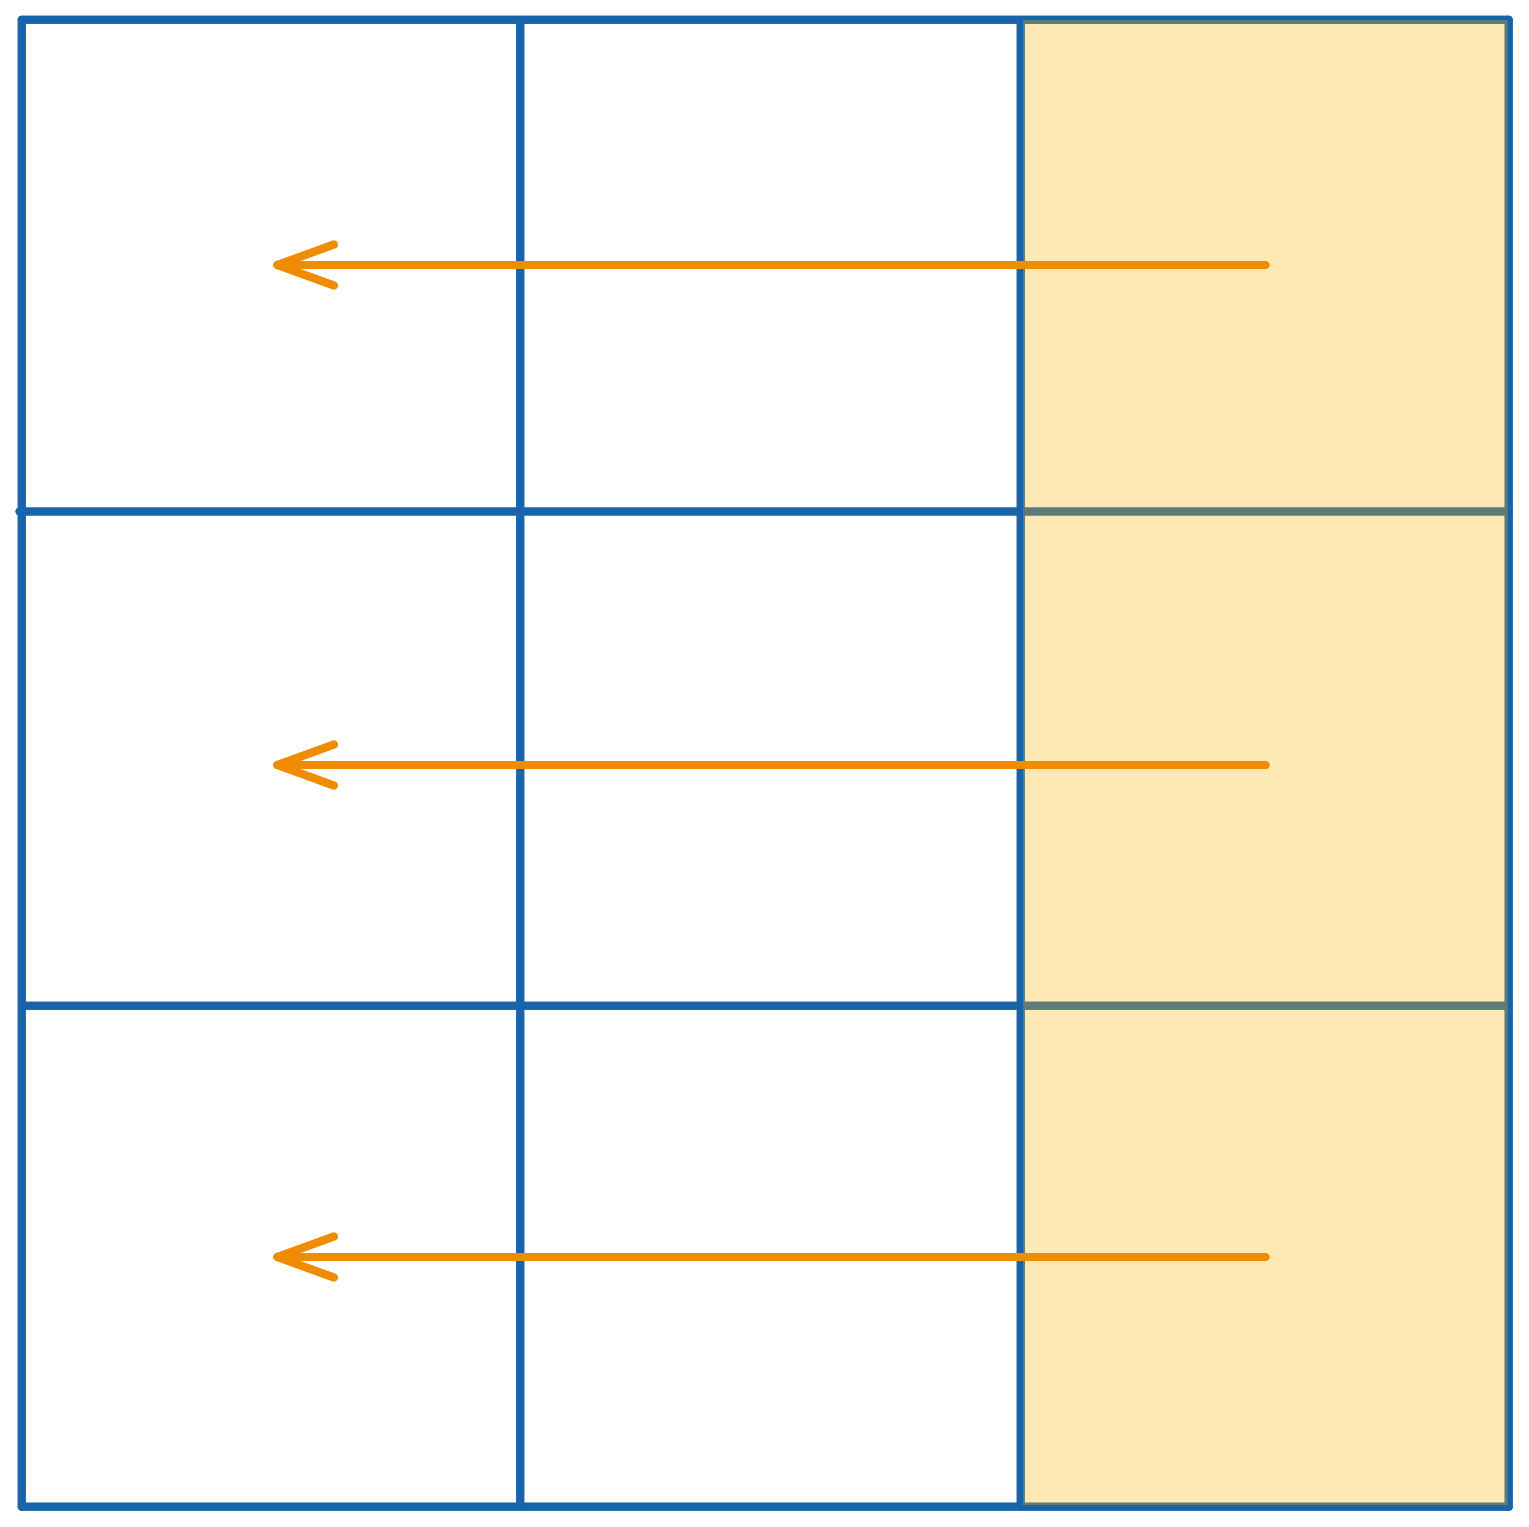
\includegraphics[width=\textwidth]{anisotropic-filtering-x-neg.png}
        \end{subfigure}
        \begin{subfigure}{.24\textwidth}
            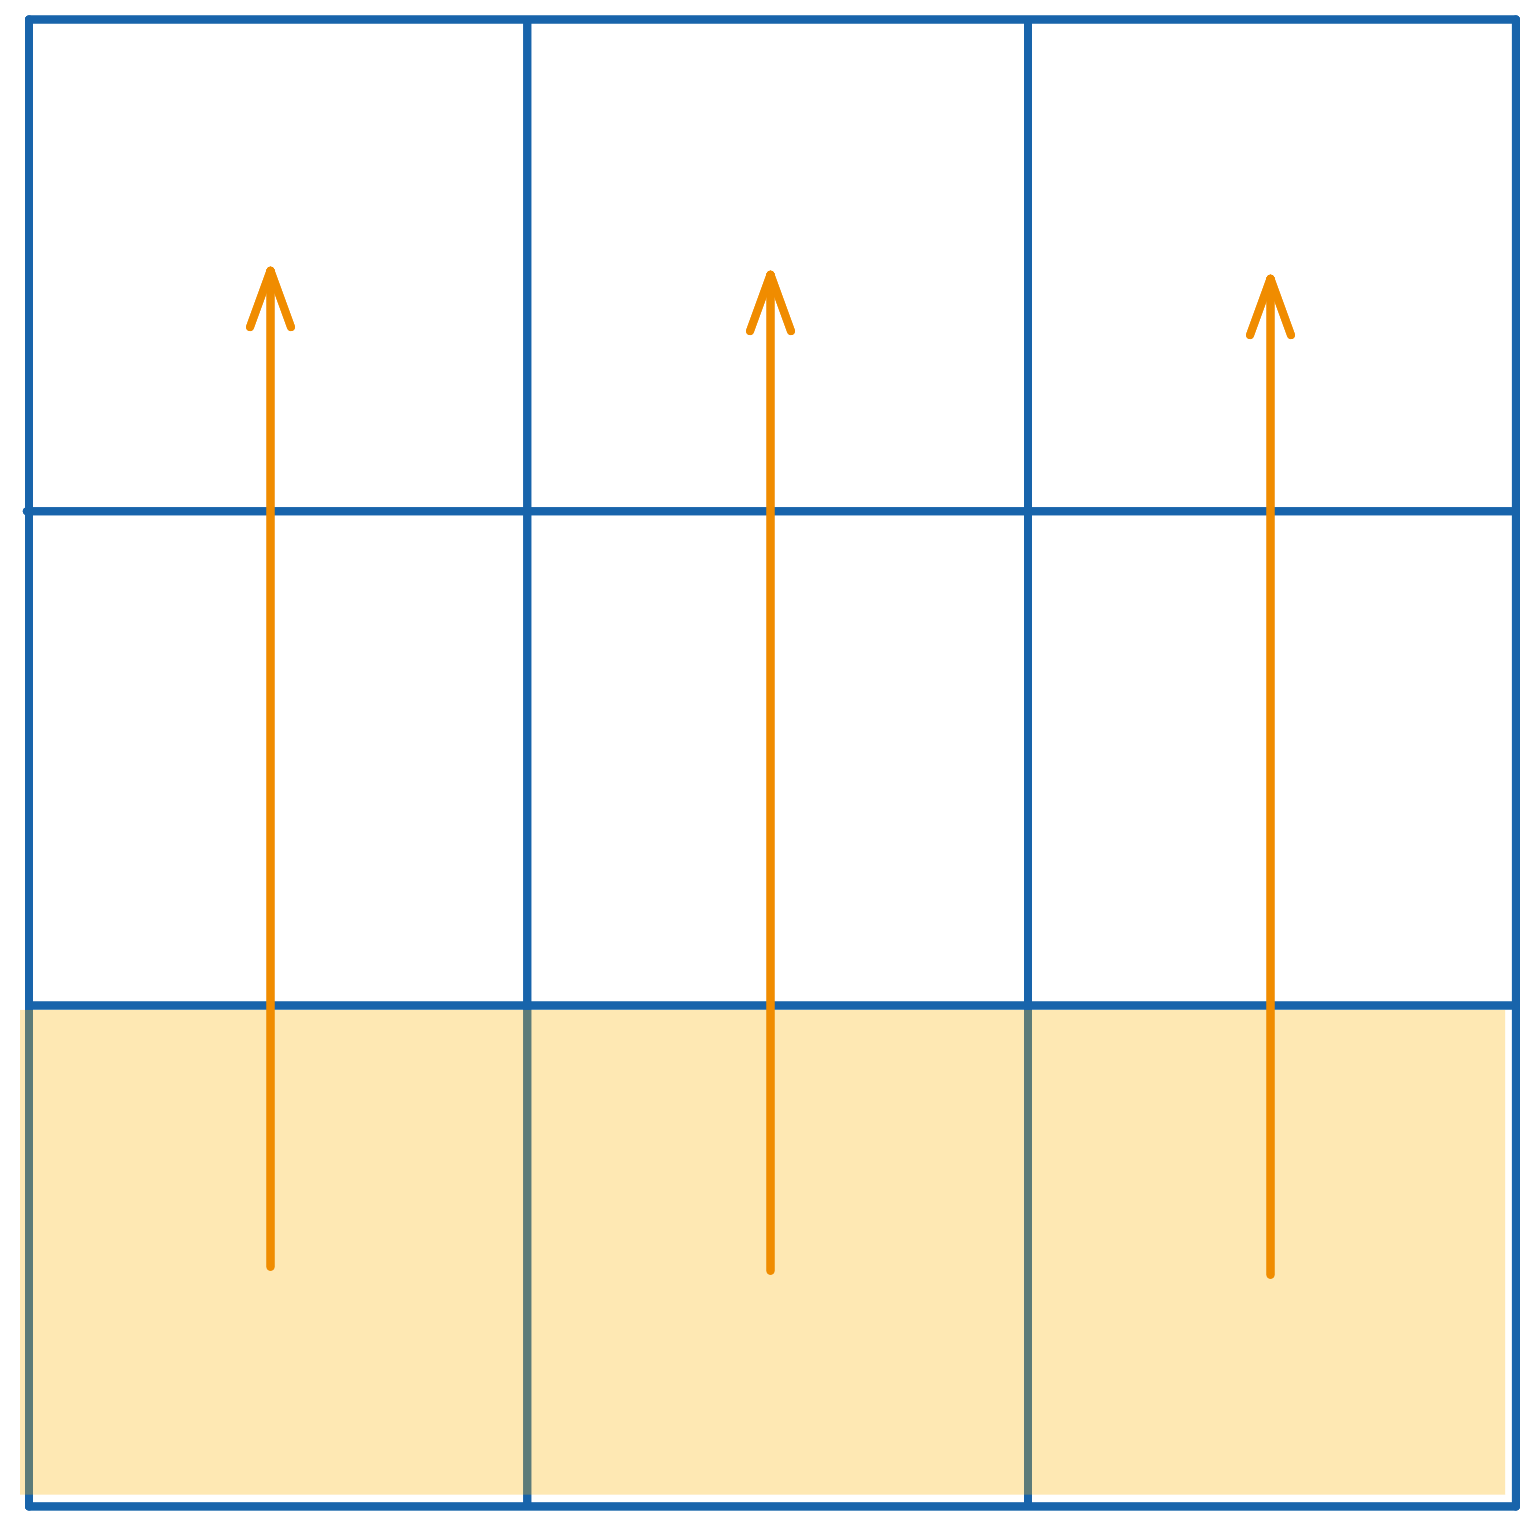
\includegraphics[width=\textwidth]{anisotropic-filtering-y.png}
        \end{subfigure}
        \begin{subfigure}{.24\textwidth}
            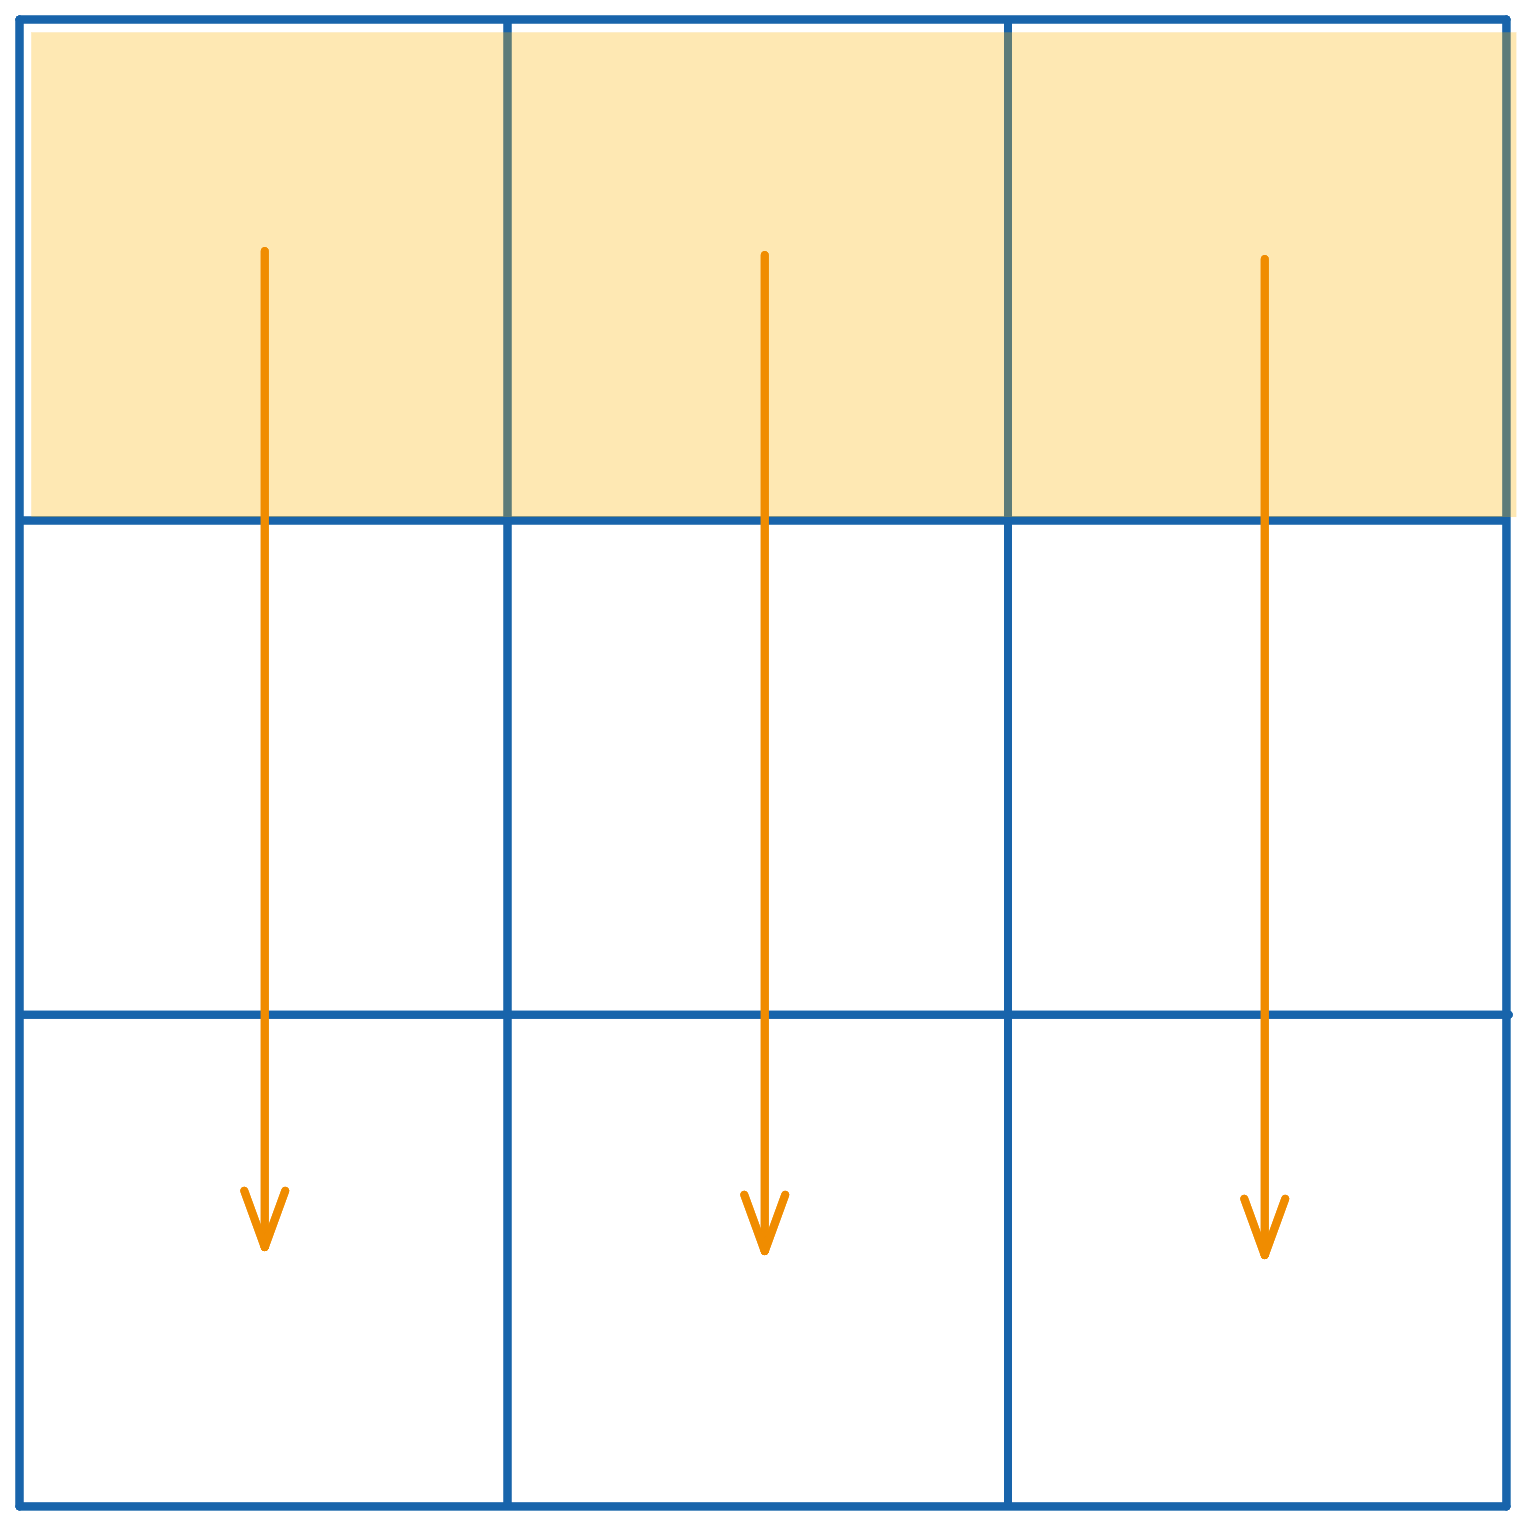
\includegraphics[width=\textwidth]{anisotropic-filtering-y-neg.png}
        \end{subfigure}
    \end{center}
    \caption{Filtrado anisotrópico en todas las direcciones.}
    \label{fig:svo_filtering_anisotropic}
\end{figure}

El filtrado anisotrópico soluciona situaciones como la de la pared mencionada anteriormente.
Para el caso de la pared fina, el vóxel que contiene la pared es opaco en la dirección paralela a la normal de la pared y prácticamente transparente en cualquiera de las perpendiculares.

\section{Inyección de fotones}\label{sec:photon-injection}

Hasta ahora tenemos la estructura de datos creada, conteniendo el color y opacidad de toda la escena en las hojas y un promedio de los niveles inferiores en todos los nodos interiores.
El objetivo del algoritmo es la iluminación global de una escena, por lo que necesitamos información de la luz.
En este paso, lanzamos fotones a partir de la fuente de luz de la escena, similar a como se hace en \textit{photon mapping}, pero utilizando el ducto de rasterización.

Se rasteriza la escena desde el punto de vista de la luz para generar una textura 2D.
En lugar de tener colores en cada téxel de la textura, se almacenan las posiciones de los objetos de la escena.
La existencia de una posición en un texel de la textura significa que esa posición es visible desde la luz, por lo que debe recibir un fotón.
Las posiciones son utilizadas para recorrer el octree y almacenar los fotones en vóxeles de sus hojas.

Los fotones que se almacenan en los vóxeles del árbol, la \textbf{irradiancia}, es el flujo lumínico recibido por cada superficie.
Luego pasan por el mismo proceso de \textit{border\_transfer} y filtrado que el color.
El \textit{border\_transfer} suma en lugar de promediar en este caso, dado que ambos lados de la frontera aportan a la cantidad de fotones total.
El filtrado funciona de la misma manera.

La etapa de construcción debe realizarse solo una vez, mientras que, al soportar luces dinámicas, esta etapa debe ejecutarse cada vez que la luz se mueva.
En esos casos, toda la irradiancia del árbol vuelve a cero y se vuelve a correr el programa que lanza los fotones, y lo llamaremos la actualización de la estructura.

% TODO: Quedó extremadamente corta esta parte.
% Estaría bueno hablar de las optimizaciones? Te hacen perder un poco.
% Suena a que las optimizaciones irían mejor en implementación.
% Un diagrama puede servir.

\section{\textit{Cone tracing}}\label{sec:cone_tracing}

Como se comentó brevemente al inicio del capítulo, el trazado de conos se realiza en el \textit{fragment shader} del ducto de rasterización.
La entrada al algoritmo de \textit{cone tracing} son los \textit{geometry buffers} que contienen los valores de la escena, ya habiendo descartado los vértices fuera de vista.
El algoritmo de trazado de conos es ejecutado para cada píxel de los geometry buffers para calcular el color final.

Dado un punto de origen $p$, se lanza uno o varios conos con cierta dirección y apertura, dependiendo del efecto que se quiera lograr.
Para cada cono, se parte desde su origen y se avanza en la dirección de su eje tomando pasos de cierto tamaño variable.
Esto se conoce como \textit{ray marching}. % TODO: No se si está bueno poner el nombre sin haberlo mencionado antes

Se toma un paso de tamaño $d$ a lo largo del eje del cono y se consigue un nuevo punto $p + d$.
Se calcula el diámetro del cono en ese punto, $h$.
Luego se encuentra el nivel del octree $i$ con el menor tamaño posible de vóxel que sea mayor al diámetro del cono $h$.
Dado ese nivel $i$ y la posición del punto $p + d$, se recorre el octree y se encuentra el nodo correspondiente a ese nivel que incluye el punto.
Ese nodo tiene un brick asociado, cuyos vóxeles tienen los valores prefiltrados, conseguidos en \ref{design:filtering}.
Se usa el valor del vóxel que contiene al punto $p + d$, este valor es una muestra $m$.

Este proceso se vuelve a repetir.
Se toma un nuevo paso, con un largo potencialmente diferente, $d'$ y se llega a un nuevo punto $p + d + d'$.
Se halla el diámetro del cono en ese punto, $h'$.
Se halla el nivel del octree $i'$, el brick, el vóxel que contiene el punto y su valor es una segunda muestra $m'$.

Estas muestras se acumulan a lo largo del cono.
En caso de vóxeles anisotrópicos, también depende de la dirección del eje del cono.
Se sigue avanzando paso a paso acumulando valores hasta satisfacer un criterio de parada,
que puede ser llegar a un máximo valor acumulado, o haber recorrido una distancia máxima a lo largo del eje del cono.

Este algoritmo se puede observar en la figura \ref{fig:cone-tracing-sampling}.

\begin{figure}
    \begin{subfigure}{.49\textwidth}
        \centering
        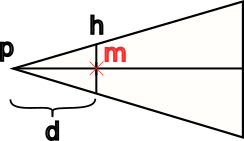
\includegraphics[width=.75\textwidth]{cone-tracing-first.png}
        \caption{Toma de una primer muestra $m$.}
    \end{subfigure}
    \begin{subfigure}{.49\textwidth}
        \centering
        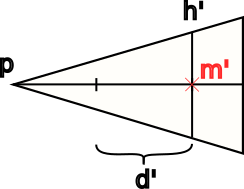
\includegraphics[width=.75\textwidth]{cone-tracing-second.png}
        \caption{Toma de una segunda muestra $m'$.}
    \end{subfigure}
    \caption{Toma de muestras a lo largo del cono en \textit{cone tracing}.}
    \label{fig:cone-tracing-sampling}
\end{figure}

Para calcular luz indirecta, las muestras son un color $c$ y una opacidad $\alpha$.
Si en cada paso consideramos $c$ y $\alpha$ como los valores hasta el momento, y $c'$ y $\alpha'$ como los valores de la nueva muestra $m'$, entonces en cada paso los valores de $c$ y $\alpha$ se calculan de la siguiente manera (\cite{voxel-cone-tracing}):

$$
\begin{cases}
    c = \alpha c + (1 - \alpha) \alpha' c' \\
    \alpha = \alpha + (1 - \alpha) \alpha'
\end{cases}
$$

Para la luz indirecta difusa, se lanzan conos para cubrir el hemisferio centrado en la normal del punto, como se puede ver en la figura \ref{fig:cone-hemisphere}.
En la mayoría de los casos, 5 conos anchos difusos dan un buen resultado.
Cada cono acumula el color de los vóxeles con los que se encuentra multiplicado por la cantidad de fotones, que fue almacenada en el paso de inyección de fotones (\ref{sec:photon-injection}).
Esto logra un efecto de \textit{color bleeding}, donde las superficies adquieren color de otras superficies cercanas que reciben y dispersan luz.

\begin{figure}[hb]
    \centering
    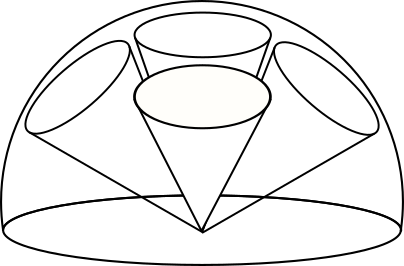
\includegraphics[width=.25\textwidth]{cones-on-hemisphere.png}
    \caption{Conos intentando cubrir el hemisferio en dirección de $n$, centrado en $p$.}
    \label{fig:cone-hemisphere}
\end{figure}

Para la luz indirecta especular, se lanza un solo cono fino en la dirección de reflexión.
El cono, al ser más fino, es rápidamente ocluido por nodos de niveles más bajos, con lo que el reflejo tiene mejor definición.
Si se utiliza un mayor ángulo de apertura del cono, el reflejo se ve más turbio, simulando una superficie menos pulida.

\section{Oclusión ambiental}

La oclusión ambiental es una técnica de rendering que se usa para calcular qué tan expuesto está cada punto de una escena a la luz ambiental.
\textit{Cone tracing} se puede usar para calcular este valor.
El efecto no aporta más al realismo de una escena una vez que se usan técnicas de iluminación indirecta, pero es un buen paso previo para ver el funcionamiento del algoritmo.

Para calcularlo, se lanzan varios conos, cubriendo el hemisferio centrado en la normal de la superficie en el punto.
El único valor necesario es la opacidad.
A medida que se viaja a lo largo de un cono, se va acumulando la opacidad de los vóxeles correspondientes.
Se define una distancia máxima y el criterio de parada es cuando el punto a lo largo del cono pasa esa distancia máxima, o la oclusión llega a 1.

\section{Conos de sombra}

De la misma manera que el trazado de rayos logra sombras lanzando un rayo hacia la fuente de luz, \textit{cone tracing} lo logra lanzando un cono hacia la fuente de luz.
El cono toma en cuenta únicamente la opacidad y su criterio de parada es alcanzar la luz o 1 de opacidad antes.
El beneficio de que sea un cono en lugar de un rayo, y de tener la estructura jerárquica del \textit{octree}, es que se logran sombras suaves, sin necesidad de lanzar varios y promediar sus resultados.

% END.
